\documentclass[]{book}
\usepackage{lmodern}
\usepackage{amssymb,amsmath}
\usepackage{ifxetex,ifluatex}
\usepackage{fixltx2e} % provides \textsubscript
\ifnum 0\ifxetex 1\fi\ifluatex 1\fi=0 % if pdftex
  \usepackage[T1]{fontenc}
  \usepackage[utf8]{inputenc}
\else % if luatex or xelatex
  \ifxetex
    \usepackage{mathspec}
  \else
    \usepackage{fontspec}
  \fi
  \defaultfontfeatures{Ligatures=TeX,Scale=MatchLowercase}
\fi
% use upquote if available, for straight quotes in verbatim environments
\IfFileExists{upquote.sty}{\usepackage{upquote}}{}
% use microtype if available
\IfFileExists{microtype.sty}{%
\usepackage{microtype}
\UseMicrotypeSet[protrusion]{basicmath} % disable protrusion for tt fonts
}{}
\usepackage[margin=1in]{geometry}
\usepackage{hyperref}
\hypersetup{unicode=true,
            pdftitle={Slow ggplot2},
            pdfauthor={Evangeline Reynolds},
            pdfborder={0 0 0},
            breaklinks=true}
\urlstyle{same}  % don't use monospace font for urls
\usepackage{natbib}
\bibliographystyle{apalike}
\usepackage{color}
\usepackage{fancyvrb}
\newcommand{\VerbBar}{|}
\newcommand{\VERB}{\Verb[commandchars=\\\{\}]}
\DefineVerbatimEnvironment{Highlighting}{Verbatim}{commandchars=\\\{\}}
% Add ',fontsize=\small' for more characters per line
\usepackage{framed}
\definecolor{shadecolor}{RGB}{248,248,248}
\newenvironment{Shaded}{\begin{snugshade}}{\end{snugshade}}
\newcommand{\KeywordTok}[1]{\textcolor[rgb]{0.13,0.29,0.53}{\textbf{#1}}}
\newcommand{\DataTypeTok}[1]{\textcolor[rgb]{0.13,0.29,0.53}{#1}}
\newcommand{\DecValTok}[1]{\textcolor[rgb]{0.00,0.00,0.81}{#1}}
\newcommand{\BaseNTok}[1]{\textcolor[rgb]{0.00,0.00,0.81}{#1}}
\newcommand{\FloatTok}[1]{\textcolor[rgb]{0.00,0.00,0.81}{#1}}
\newcommand{\ConstantTok}[1]{\textcolor[rgb]{0.00,0.00,0.00}{#1}}
\newcommand{\CharTok}[1]{\textcolor[rgb]{0.31,0.60,0.02}{#1}}
\newcommand{\SpecialCharTok}[1]{\textcolor[rgb]{0.00,0.00,0.00}{#1}}
\newcommand{\StringTok}[1]{\textcolor[rgb]{0.31,0.60,0.02}{#1}}
\newcommand{\VerbatimStringTok}[1]{\textcolor[rgb]{0.31,0.60,0.02}{#1}}
\newcommand{\SpecialStringTok}[1]{\textcolor[rgb]{0.31,0.60,0.02}{#1}}
\newcommand{\ImportTok}[1]{#1}
\newcommand{\CommentTok}[1]{\textcolor[rgb]{0.56,0.35,0.01}{\textit{#1}}}
\newcommand{\DocumentationTok}[1]{\textcolor[rgb]{0.56,0.35,0.01}{\textbf{\textit{#1}}}}
\newcommand{\AnnotationTok}[1]{\textcolor[rgb]{0.56,0.35,0.01}{\textbf{\textit{#1}}}}
\newcommand{\CommentVarTok}[1]{\textcolor[rgb]{0.56,0.35,0.01}{\textbf{\textit{#1}}}}
\newcommand{\OtherTok}[1]{\textcolor[rgb]{0.56,0.35,0.01}{#1}}
\newcommand{\FunctionTok}[1]{\textcolor[rgb]{0.00,0.00,0.00}{#1}}
\newcommand{\VariableTok}[1]{\textcolor[rgb]{0.00,0.00,0.00}{#1}}
\newcommand{\ControlFlowTok}[1]{\textcolor[rgb]{0.13,0.29,0.53}{\textbf{#1}}}
\newcommand{\OperatorTok}[1]{\textcolor[rgb]{0.81,0.36,0.00}{\textbf{#1}}}
\newcommand{\BuiltInTok}[1]{#1}
\newcommand{\ExtensionTok}[1]{#1}
\newcommand{\PreprocessorTok}[1]{\textcolor[rgb]{0.56,0.35,0.01}{\textit{#1}}}
\newcommand{\AttributeTok}[1]{\textcolor[rgb]{0.77,0.63,0.00}{#1}}
\newcommand{\RegionMarkerTok}[1]{#1}
\newcommand{\InformationTok}[1]{\textcolor[rgb]{0.56,0.35,0.01}{\textbf{\textit{#1}}}}
\newcommand{\WarningTok}[1]{\textcolor[rgb]{0.56,0.35,0.01}{\textbf{\textit{#1}}}}
\newcommand{\AlertTok}[1]{\textcolor[rgb]{0.94,0.16,0.16}{#1}}
\newcommand{\ErrorTok}[1]{\textcolor[rgb]{0.64,0.00,0.00}{\textbf{#1}}}
\newcommand{\NormalTok}[1]{#1}
\usepackage{longtable,booktabs}
\usepackage{graphicx,grffile}
\makeatletter
\def\maxwidth{\ifdim\Gin@nat@width>\linewidth\linewidth\else\Gin@nat@width\fi}
\def\maxheight{\ifdim\Gin@nat@height>\textheight\textheight\else\Gin@nat@height\fi}
\makeatother
% Scale images if necessary, so that they will not overflow the page
% margins by default, and it is still possible to overwrite the defaults
% using explicit options in \includegraphics[width, height, ...]{}
\setkeys{Gin}{width=\maxwidth,height=\maxheight,keepaspectratio}
\IfFileExists{parskip.sty}{%
\usepackage{parskip}
}{% else
\setlength{\parindent}{0pt}
\setlength{\parskip}{6pt plus 2pt minus 1pt}
}
\setlength{\emergencystretch}{3em}  % prevent overfull lines
\providecommand{\tightlist}{%
  \setlength{\itemsep}{0pt}\setlength{\parskip}{0pt}}
\setcounter{secnumdepth}{5}
% Redefines (sub)paragraphs to behave more like sections
\ifx\paragraph\undefined\else
\let\oldparagraph\paragraph
\renewcommand{\paragraph}[1]{\oldparagraph{#1}\mbox{}}
\fi
\ifx\subparagraph\undefined\else
\let\oldsubparagraph\subparagraph
\renewcommand{\subparagraph}[1]{\oldsubparagraph{#1}\mbox{}}
\fi

%%% Use protect on footnotes to avoid problems with footnotes in titles
\let\rmarkdownfootnote\footnote%
\def\footnote{\protect\rmarkdownfootnote}

%%% Change title format to be more compact
\usepackage{titling}

% Create subtitle command for use in maketitle
\newcommand{\subtitle}[1]{
  \posttitle{
    \begin{center}\large#1\end{center}
    }
}

\setlength{\droptitle}{-2em}
  \title{Slow ggplot2}
  \pretitle{\vspace{\droptitle}\centering\huge}
  \posttitle{\par}
  \author{Evangeline Reynolds}
  \preauthor{\centering\large\emph}
  \postauthor{\par}
  \predate{\centering\large\emph}
  \postdate{\par}
  \date{2018-09-29}

\usepackage{booktabs}

\usepackage{amsthm}
\newtheorem{theorem}{Theorem}[chapter]
\newtheorem{lemma}{Lemma}[chapter]
\theoremstyle{definition}
\newtheorem{definition}{Definition}[chapter]
\newtheorem{corollary}{Corollary}[chapter]
\newtheorem{proposition}{Proposition}[chapter]
\theoremstyle{definition}
\newtheorem{example}{Example}[chapter]
\theoremstyle{definition}
\newtheorem{exercise}{Exercise}[chapter]
\theoremstyle{remark}
\newtheorem*{remark}{Remark}
\newtheorem*{solution}{Solution}
\begin{document}
\maketitle

{
\setcounter{tocdepth}{1}
\tableofcontents
}
\chapter{Introduction}\label{intro}

In late 2016 I heard Andy Kreibel (and \_\_) being interviewed on the
Podcast ``Data Stories''. He was invited onto the show because he had
started the initiative \#MakeoverMonday, in which he would find the data
for an existing data visualization that he had come across in the media,
and would recreate the visualization using Tableau, a tool that they
were both expert in, but found that they weren't practicing as regularly
due to the grind of administrative jobs. The two friends shared their
makeovers products with each other, but also with the world on Twitter.
Soon, more people expressed interest in joining, and they two started a
more organized initiative - posting the original graph and data every
Sunday, so that whoever wanted to could participate in \#Makeovermonday.

My first submission was late 2016, after catching wind of the exciting
project via the podcast. I made a scrappy little graph about motorway
casualties; sad topic, but fun graph making.

I was using base R at that time. Then in the summer of 2017 I went to a
conference in Zurich, the women's summer school for political
methodology. There was a session on ggplot2. I internalized some of the
basics, and decided that if I wanted to learn that (powerful - as
everyone kept calling it) graphing system, then I could do it via the
\#MakeoverMonday weekly exercises (not that I particpated weekly). Even
though most folks were using Tablaeu, the administrators didn't seem to
mind a few R and ggplot submission here and there. I got a little
hooked.

Early this year Andy and Eva Murry sent a number of the participants a
private message on Twitter. ``We're writing a book: \#MakeoverMonday''.
They were putting together a collection of a visualizations that
resulted from the project, and were seeking perspectives of participants
as well as permission to use some of the visualizations produced for the
initiatives. Cool. I was pleased to participate. For me \#MakeoverMonday
allowed me to focus on the visualization task. Usually visualization
comes at the end of, sometimes arguous, data cleaning --- and you might
already be a little spent. Having rather clean data delivered, and
seeing the approaches of many other (many brilliant) data visualizers
was a treat. I still need to buy my copy of the book, which contains a
visualization of food prices in London as a function of how far a
restaurant is from the Big Ben.

And now, using the magic of RStudio and Yihui Xie's bookdown, I'm
putting together my own little collection. Of course there is a bit of
curation involved --- I'm not including every plot. And, I'm revising
the exact code that creates the plots in many cases, to be more
consistent across plots, and also, I think, to make communicating about
how the plot was built easy. This involves:

\begin{itemize}
\tightlist
\item
  using fewer functions (labs(title = ) instead of ggtitle())
\item
  pulling out aes() from the ggplot() function
\item
  multiply using functions aes(x = ?) + aes(y = ?) rather than aes(x = ,
  y = )
\item
  using base R functions and tidyverse functions. For other packages,
  the :: style to call them
\item
  write out arguments (no shortcuts) aes(x = gdppercap) not
  aes(gdppercap)
\item
  order ggplot commands so that reactivity is obvious
\end{itemize}

\chapter{Baseball, WAR, and Ethnicity}\label{baseball-war-and-ethnicity}

This data visualization uses the WAR measure in baseball, a calculation
based on the contributions of players. The visualizations show that new
ethnicities and races started to be included in Major League baseball,
the minority players that joined tended to contribute more than the
expected value for players overall. For example, from 1947, when Jackie
Robinson joined Major League baseball, and onward, the percent of
African American players was outpaced by the percent calculated
contributions (WAR) of African American players.

A random sample from the data set:

\begin{tabular}{r|l|l|r}
\hline
Year & Ethnicity & type & Percent\\
\hline
1983 & African American & \% of WAR & 25.8\\
\hline
1949 & African American & \% of Players & 1.5\\
\hline
1950 & Latino & \% of WAR & 1.7\\
\hline
1967 & Latino & \% of Players & 10.7\\
\hline
1978 & Asian & \% of WAR & 0.0\\
\hline
\end{tabular}

\begin{Shaded}
\begin{Highlighting}[]
\KeywordTok{ggplot}\NormalTok{(df_gather) }\OperatorTok{+}
\StringTok{  }\KeywordTok{aes}\NormalTok{(}\DataTypeTok{x =}\NormalTok{ Year) }\OperatorTok{+}
\StringTok{  }\KeywordTok{aes}\NormalTok{(}\DataTypeTok{y =}\NormalTok{ Percent) }\OperatorTok{+}
\StringTok{  }\KeywordTok{aes}\NormalTok{(}\DataTypeTok{fill =}\NormalTok{ type) }\OperatorTok{+}
\StringTok{  }\KeywordTok{facet_wrap}\NormalTok{(}\OperatorTok{~}\StringTok{ }\NormalTok{Ethnicity) }\OperatorTok{+}
\StringTok{  }\KeywordTok{geom_area}\NormalTok{(}\DataTypeTok{alpha =}\NormalTok{ .}\DecValTok{5}\NormalTok{, }\DataTypeTok{position =} \StringTok{"dodge"}\NormalTok{) }\OperatorTok{+}
\StringTok{  }\KeywordTok{labs}\NormalTok{(}\DataTypeTok{fill =} \StringTok{""}\NormalTok{) }\OperatorTok{+}
\StringTok{  }\KeywordTok{labs}\NormalTok{(}\DataTypeTok{x =} \StringTok{""}\NormalTok{) }\OperatorTok{+}
\StringTok{  }\KeywordTok{labs}\NormalTok{(}\DataTypeTok{title =} \StringTok{"American Baseball Demographics 1947-2016"}\NormalTok{) }\OperatorTok{+}
\StringTok{  }\KeywordTok{labs}\NormalTok{(}\DataTypeTok{subtitle =} \StringTok{"Percentage of players and WAR percentage (WAR is a calculation of value contributed)}\CharTok{\textbackslash{}n}\StringTok{Data: SABR.org | Vis: @EvaMaeRey for #MakeoverMonday"}\NormalTok{) }\OperatorTok{+}
\StringTok{  }\KeywordTok{theme_light}\NormalTok{() }
\end{Highlighting}
\end{Shaded}

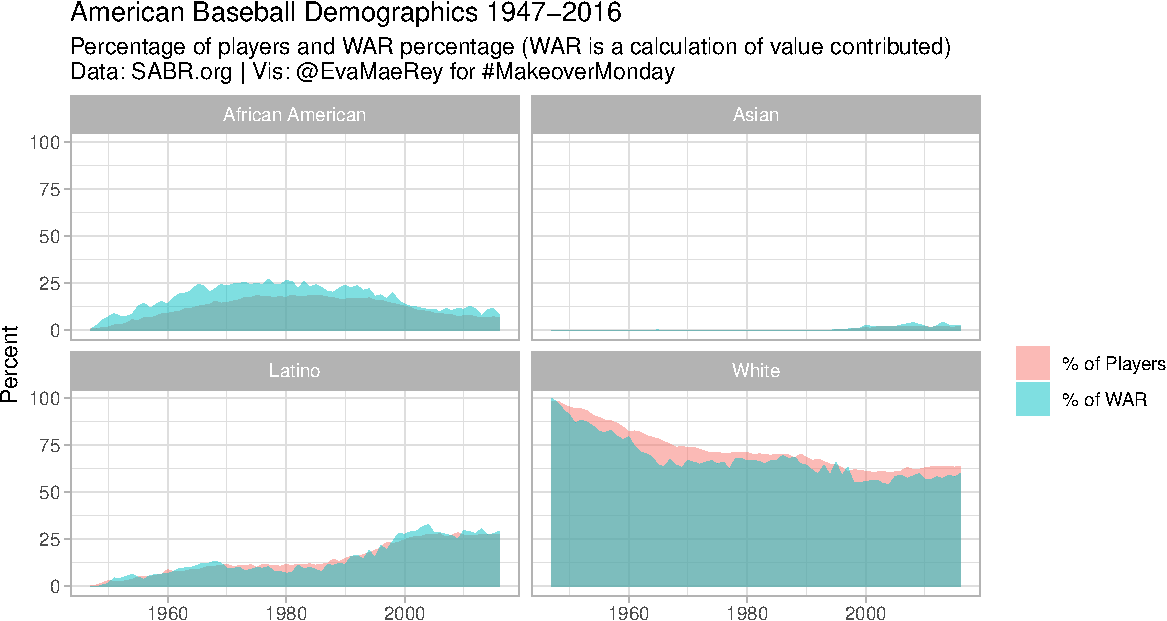
\includegraphics{makeovermonday_book_files/figure-latex/unnamed-chunk-6-1.pdf}

\chapter{Christmas Trees}\label{christmas-trees}

Here is a simple plot of Christmas Tree Sales in the U.S. The plot shows
that artificial tree sales are on the rise, contrasting with declines in
real trees. The title plays on the German Christmas Carol ``O
Tannenbaum'', ``Oh Christmas Tree'' in English. ``Wie echt sind deine
Blätter?'' means ``how real are your leaves''; the original text from
the carol is ``Wie treu sind deine Blätter!'' which means ``How true
your leaves are!''

I also plot the cumulative number of trees purchased of each type,
artificial and real, from 2004 to 2014, comparing that to the 2016 U.S.
population. Almost one real tree per person was bought over the course
of 10 years!

A random sample from the data set:

\begin{tabular}{r|r|l|r}
\hline
Year & Number of trees sold & Type of tree & Number of trees sold (millions)\\
\hline
2008 & 11700000 & Fake tree & 11.7\\
\hline
2011 & 9500000 & Fake tree & 9.5\\
\hline
2012 & 10900000 & Fake tree & 10.9\\
\hline
2015 & 25900000 & Real tree & 25.9\\
\hline
2006 & 9300000 & Fake tree & 9.3\\
\hline
\end{tabular}

\begin{Shaded}
\begin{Highlighting}[]
\KeywordTok{ggplot}\NormalTok{(}\DataTypeTok{data =}\NormalTok{ dta) }\OperatorTok{+}
\StringTok{  }\KeywordTok{aes}\NormalTok{(Year) }\OperatorTok{+}
\StringTok{  }\KeywordTok{aes}\NormalTok{(}\DataTypeTok{y =} \StringTok{`}\DataTypeTok{Number of trees sold (millions)}\StringTok{`}\NormalTok{) }\OperatorTok{+}
\StringTok{  }\KeywordTok{geom_point}\NormalTok{() }\OperatorTok{+}
\StringTok{  }\KeywordTok{aes}\NormalTok{(}\DataTypeTok{col =} \KeywordTok{fct_rev}\NormalTok{(}\StringTok{`}\DataTypeTok{Type of tree}\StringTok{`}\NormalTok{)) }\OperatorTok{+}
\StringTok{  }\KeywordTok{geom_smooth}\NormalTok{(}\DataTypeTok{method =} \StringTok{"lm"}\NormalTok{, }\DataTypeTok{se =}\NormalTok{ F) }\OperatorTok{+}
\StringTok{  }\KeywordTok{scale_color_manual}\NormalTok{(}\DataTypeTok{values =} \KeywordTok{c}\NormalTok{(}\StringTok{"darkgreen"}\NormalTok{, }\StringTok{"green"}\NormalTok{)) }\OperatorTok{+}
\StringTok{  }\KeywordTok{ylim}\NormalTok{(}\KeywordTok{c}\NormalTok{(}\DecValTok{0}\NormalTok{, }\DecValTok{35}\NormalTok{)) }\OperatorTok{+}
\StringTok{  }\KeywordTok{labs}\NormalTok{(}\DataTypeTok{col =} \StringTok{""}\NormalTok{) }\OperatorTok{+}
\StringTok{  }\KeywordTok{labs}\NormalTok{(}\DataTypeTok{title =} \StringTok{"Wie echt sind deine Blätter?"}\NormalTok{) }\OperatorTok{+}
\StringTok{  }\KeywordTok{labs}\NormalTok{(}\DataTypeTok{subtitle =} \StringTok{"Real and fake Christmas trees sold in the US | Data Source: Statista | @EvaMaeRey "}\NormalTok{) }\OperatorTok{+}
\StringTok{  }\KeywordTok{theme_bw}\NormalTok{() }
\end{Highlighting}
\end{Shaded}

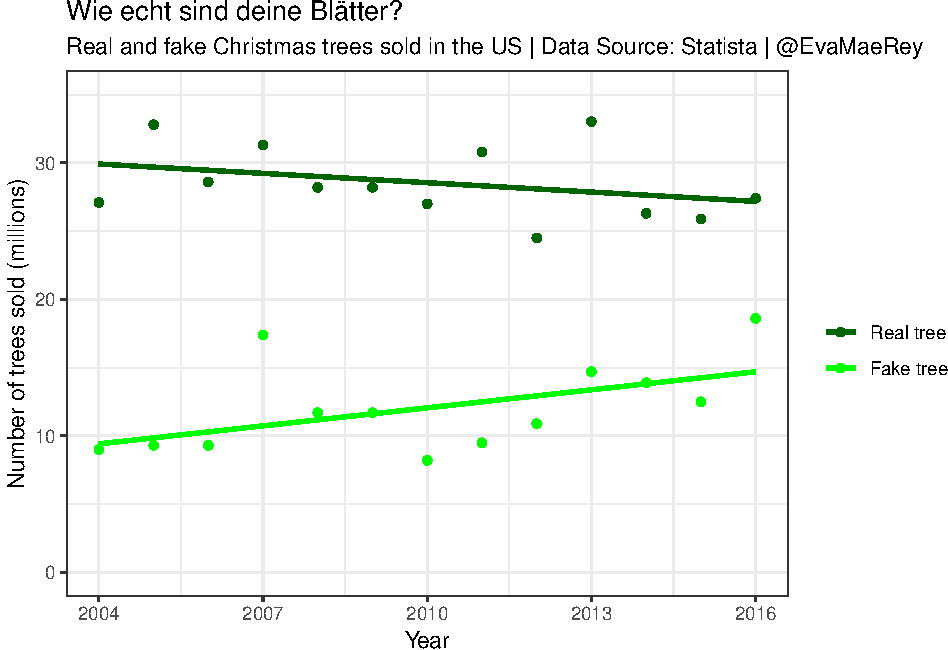
\includegraphics{makeovermonday_book_files/figure-latex/unnamed-chunk-9-1.pdf}

\begin{Shaded}
\begin{Highlighting}[]
\NormalTok{dta <-}\StringTok{ }\NormalTok{dta }\OperatorTok
\StringTok{  }\KeywordTok{group_by}\NormalTok{(}\StringTok{`}\DataTypeTok{Type of tree}\StringTok{`}\NormalTok{) }\OperatorTok
\StringTok{  }\KeywordTok{mutate}\NormalTok{(}\DataTypeTok{cumula =} \KeywordTok{cumsum}\NormalTok{(}\StringTok{`}\DataTypeTok{Number of trees sold (millions)}\StringTok{`}\NormalTok{))}

\KeywordTok{ggplot}\NormalTok{(dta }\OperatorTok\StringTok{ }\KeywordTok{filter}\NormalTok{(Year }\OperatorTok{<=}\StringTok{ }\DecValTok{2014}\NormalTok{)) }\OperatorTok{+}
\StringTok{  }\KeywordTok{aes}\NormalTok{(Year) }\OperatorTok{+}\StringTok{ }
\StringTok{  }\KeywordTok{aes}\NormalTok{(}\DataTypeTok{y =}\NormalTok{ cumula) }\OperatorTok{+}\StringTok{ }
\StringTok{  }\KeywordTok{aes}\NormalTok{(}\DataTypeTok{fill =} \StringTok{`}\DataTypeTok{Type of tree}\StringTok{`}\NormalTok{) }\OperatorTok{+}
\StringTok{  }\KeywordTok{geom_hline}\NormalTok{(}\DataTypeTok{yintercept =} \FloatTok{323.1}\NormalTok{, }\DataTypeTok{lty =} \DecValTok{2}\NormalTok{) }\OperatorTok{+}
\StringTok{  }\KeywordTok{geom_area}\NormalTok{(}\DataTypeTok{alpha =}\NormalTok{ .}\DecValTok{2}\NormalTok{) }\OperatorTok{+}\StringTok{ }\KeywordTok{facet_wrap}\NormalTok{(}\OperatorTok{~}\StringTok{ `}\DataTypeTok{Type of tree}\StringTok{`}\NormalTok{) }\OperatorTok{+}
\StringTok{  }\KeywordTok{annotate}\NormalTok{(}\DataTypeTok{geom =} \StringTok{"text"}\NormalTok{, }\DataTypeTok{x =} \DecValTok{2010}\NormalTok{, }\DataTypeTok{y =} \DecValTok{335}\NormalTok{, }\DataTypeTok{label =} \StringTok{"US Population (2016)"}\NormalTok{) }\OperatorTok{+}
\StringTok{  }\KeywordTok{labs}\NormalTok{(}\DataTypeTok{title =} \StringTok{"Ten years of trees."}\NormalTok{) }\OperatorTok{+}
\StringTok{  }\KeywordTok{labs}\NormalTok{(}\DataTypeTok{subtitle =} \StringTok{"Cummulative real and fake Christmas trees sold in the US}\CharTok{\textbackslash{}n}\StringTok{Data Source: Statista | @EvaMaeRey "}\NormalTok{) }\OperatorTok{+}
\StringTok{  }\KeywordTok{scale_fill_manual}\NormalTok{(}\DataTypeTok{values =} \KeywordTok{c}\NormalTok{(}\StringTok{"green"}\NormalTok{, }\StringTok{"darkgreen"}\NormalTok{)) }\OperatorTok{+}
\StringTok{  }\KeywordTok{theme_bw}\NormalTok{() }\OperatorTok{+}
\StringTok{  }\KeywordTok{ylim}\NormalTok{(}\KeywordTok{c}\NormalTok{(}\DecValTok{0}\NormalTok{, }\DecValTok{400}\NormalTok{))}
\end{Highlighting}
\end{Shaded}

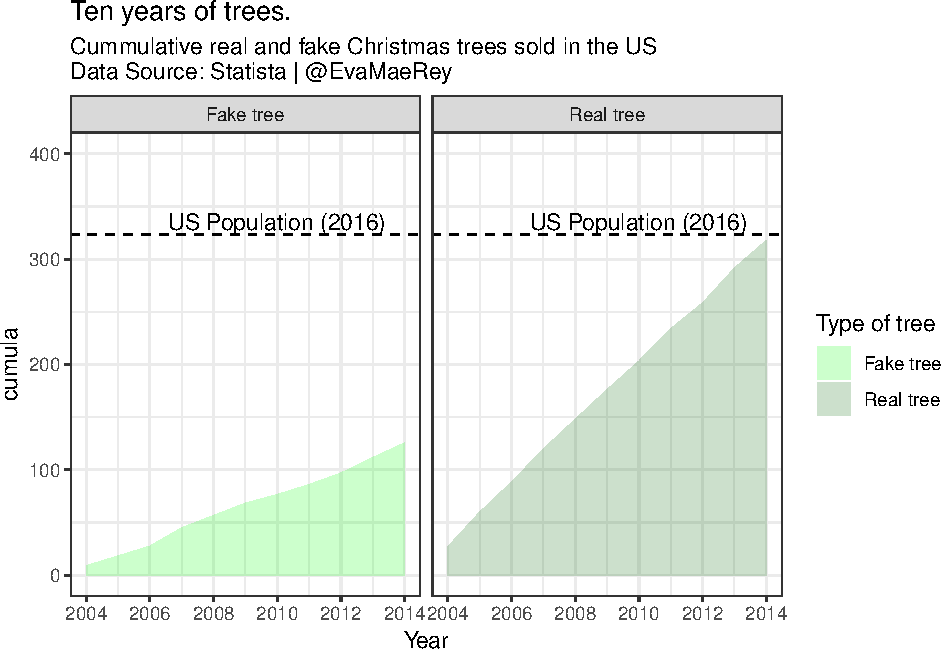
\includegraphics{makeovermonday_book_files/figure-latex/unnamed-chunk-10-1.pdf}

\chapter{Officials' beliefs about women's
representation}\label{officials-beliefs-about-womens-representation}

The data provided is based on a small survey of elite officials in five
less developed countries. The question that arrises from the data is:
How well do elites know the conditions in their countries. In general,
the elites overestimate women's representation. But this is not the case
in Senegal, where there are gender quotas in the Parliament. Most elites
therefore estimate that the representation is about equal with men. I
jitter the responses of the elites horizontally to avoid overplotting.

A random sample from the data set:

\begin{tabular}{l|l|r|l|r}
\hline
Country & Topic & value & value\_type & alpha\\
\hline
Senegal & Share of seats held by women & 0.50 & Individual belief & 0.3\\
\hline
Kenya & Share of seats held by women & 0.20 & Individual belief & 0.3\\
\hline
Senegal & Share of seats held by women & 0.50 & Individual belief & 0.3\\
\hline
Colombia & Share of seats held by women & 0.30 & Individual belief & 0.3\\
\hline
Indonesia & Share of seats held by women & 0.17 & Individual belief & 0.3\\
\hline
\end{tabular}

\begin{Shaded}
\begin{Highlighting}[]
\KeywordTok{ggplot}\NormalTok{(}\DataTypeTok{data =}\NormalTok{ df_all) }\OperatorTok{+}
\StringTok{  }\KeywordTok{aes}\NormalTok{(}\DataTypeTok{x =}\NormalTok{ Country) }\OperatorTok{+}
\StringTok{  }\KeywordTok{aes}\NormalTok{(}\DataTypeTok{y =}\NormalTok{ value) }\OperatorTok{+}
\StringTok{  }\KeywordTok{aes}\NormalTok{(}\DataTypeTok{col =} \KeywordTok{fct_inorder}\NormalTok{(value_type)) }\OperatorTok{+}
\StringTok{  }\KeywordTok{aes}\NormalTok{(}\DataTypeTok{alpha =} \KeywordTok{fct_inorder}\NormalTok{(value_type)) }\OperatorTok{+}
\StringTok{  }\KeywordTok{aes}\NormalTok{(}\DataTypeTok{shape =} \KeywordTok{fct_inorder}\NormalTok{(value_type)) }\OperatorTok{+}
\StringTok{  }\KeywordTok{geom_jitter}\NormalTok{(}\DataTypeTok{width =}\NormalTok{ .}\DecValTok{1}\NormalTok{, }\DataTypeTok{height =} \DecValTok{0}\NormalTok{, }\DataTypeTok{size =} \DecValTok{7}\NormalTok{) }\OperatorTok{+}
\StringTok{  }\KeywordTok{geom_hline}\NormalTok{(}\DataTypeTok{yintercept =} \KeywordTok{c}\NormalTok{(}\DecValTok{0}\NormalTok{, }\DecValTok{100}\NormalTok{), }\DataTypeTok{col =} \StringTok{"grey"}\NormalTok{) }\OperatorTok{+}
\StringTok{  }\KeywordTok{geom_hline}\NormalTok{(}\DataTypeTok{yintercept =} \KeywordTok{c}\NormalTok{(}\DecValTok{50}\NormalTok{), }\DataTypeTok{lty =} \DecValTok{2}\NormalTok{, }\DataTypeTok{col =} \StringTok{"grey"}\NormalTok{) }\OperatorTok{+}
\StringTok{  }\KeywordTok{theme_bw}\NormalTok{(}\DataTypeTok{base_size =} \DecValTok{20}\NormalTok{, }\DataTypeTok{base_family =} \StringTok{"Times"}\NormalTok{) }\OperatorTok{+}
\StringTok{  }\KeywordTok{scale_y_continuous}\NormalTok{(}\DataTypeTok{limits =} \KeywordTok{c}\NormalTok{(}\DecValTok{0}\NormalTok{, }\DecValTok{1}\NormalTok{), }\DataTypeTok{expand =} \KeywordTok{c}\NormalTok{(}\DecValTok{0}\NormalTok{, }\DecValTok{0}\NormalTok{), }\DataTypeTok{labels =}\NormalTok{ scales}\OperatorTok{::}\NormalTok{percent) }\OperatorTok{+}
\StringTok{  }\CommentTok{# create just one key "" mixing aesthetics}
\StringTok{  }\KeywordTok{scale_colour_manual}\NormalTok{(}\DataTypeTok{name =} \StringTok{""}\NormalTok{, }\DataTypeTok{values =} \KeywordTok{c}\NormalTok{(}\StringTok{"darkblue"}\NormalTok{, }\StringTok{"goldenrod3"}\NormalTok{, }\StringTok{"goldenrod3"}\NormalTok{)) }\OperatorTok{+}
\StringTok{  }\KeywordTok{scale_alpha_manual}\NormalTok{(}\DataTypeTok{name =} \StringTok{""}\NormalTok{, }\DataTypeTok{values =} \KeywordTok{c}\NormalTok{(}\DecValTok{1}\NormalTok{, .}\DecValTok{17}\NormalTok{, }\DecValTok{1}\NormalTok{)) }\OperatorTok{+}
\StringTok{  }\KeywordTok{scale_shape_manual}\NormalTok{(}\DataTypeTok{name =} \StringTok{""}\NormalTok{, }\DataTypeTok{values =} \KeywordTok{c}\NormalTok{(}\DecValTok{8}\NormalTok{, }\DecValTok{19}\NormalTok{, }\DecValTok{8}\NormalTok{)) }\OperatorTok{+}
\StringTok{  }\KeywordTok{annotate}\NormalTok{(}\DataTypeTok{geom =} \StringTok{"text"}\NormalTok{, }\DataTypeTok{x =} \FloatTok{4.95}\NormalTok{, }\DataTypeTok{y =}\NormalTok{ .}\DecValTok{70}\NormalTok{, }
           \DataTypeTok{label =} \KeywordTok{str_wrap}\NormalTok{(}\StringTok{"Senegal's 2010 gender parity law means it leads among these countries."}\NormalTok{, }\DecValTok{16}\NormalTok{), }\DataTypeTok{size =} \DecValTok{5}\NormalTok{, }\DataTypeTok{hjust =} \DecValTok{1}\NormalTok{) }\OperatorTok{+}
\StringTok{  }\KeywordTok{annotate}\NormalTok{(}\DataTypeTok{geom =} \StringTok{"text"}\NormalTok{, }\DataTypeTok{x =} \FloatTok{5.05}\NormalTok{, }\DataTypeTok{y =}\NormalTok{ .}\DecValTok{250}\NormalTok{, }
           \DataTypeTok{label =} \KeywordTok{str_wrap}\NormalTok{(}\StringTok{"Officials seem to be aware of the law."}\NormalTok{, }\DecValTok{10}\NormalTok{), }\DataTypeTok{size =} \DecValTok{5}\NormalTok{, }\DataTypeTok{hjust =} \DecValTok{0}\NormalTok{) }\OperatorTok{+}
\StringTok{  }\KeywordTok{labs}\NormalTok{(}\DataTypeTok{x =} \StringTok{""}\NormalTok{) }\OperatorTok{+}
\StringTok{  }\KeywordTok{labs}\NormalTok{(}\DataTypeTok{y =} \StringTok{"Seats held by women"}\NormalTok{) }\OperatorTok{+}
\StringTok{  }\KeywordTok{labs}\NormalTok{(}\DataTypeTok{title =} \StringTok{"Women in national parliaments in 2015 in five countries }\CharTok{\textbackslash{}n}\StringTok{and officials' beliefs about representation"}\NormalTok{) }\OperatorTok{+}
\StringTok{  }\KeywordTok{labs}\NormalTok{(}\DataTypeTok{subtitle =} \StringTok{"Data Source: Equal Measures 2030 | Vis: Gina Reynolds @EvaMaeRey"}\NormalTok{) }
\end{Highlighting}
\end{Shaded}

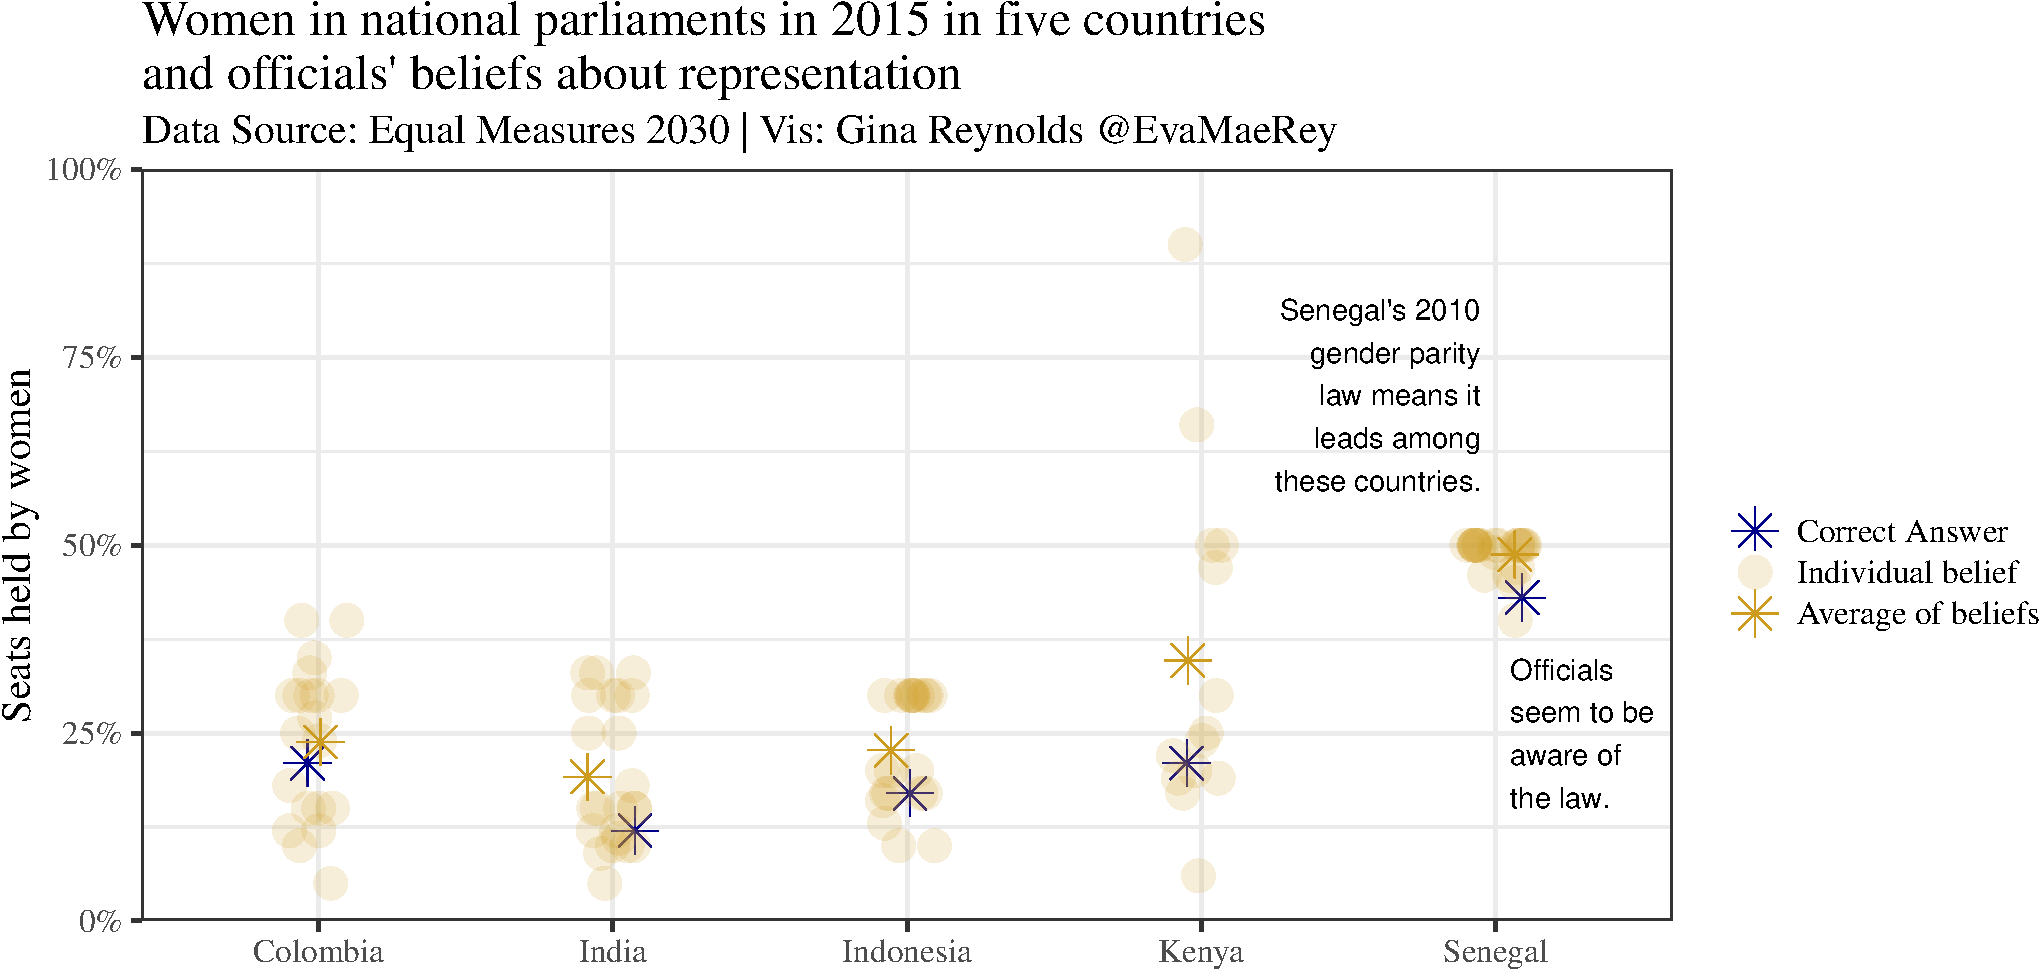
\includegraphics{makeovermonday_book_files/figure-latex/unnamed-chunk-14-1.pdf}

\chapter{Maternal Leave}\label{maternal-leave}

The OECD provides a comparative report on how much paid leave women are
entitled to after childbirth. But leave takes different forms. In some
places, the allowed leave is longer, but sometimes that means that the
pay out compared to the regular salary is lower. To emphasize the
different forms that law around paid leave take, I plotted the total
payout available to mothers as areas of rectangles, where one side is
the length of leave allowed, and the other side is the proportion of
salary paid to the new mom.

A random sample from the data set:

\begin{tabular}{l|r|r|r|r|r|r|r|r|r|l|r|r}
\hline
Country & Paid maternity leave avg payment rate (\%) & Paid maternity leave full rate equivalent in weeks & Paid maternity leave in weeks & Paid parental leave avg payment rate (\%) & Paid parental leave full rate equivalent in weeks & Paid parental leave in weeks & Total paid leave avg payment rate (\%) & Total paid leave full rate equivalent in weeks & Total paid leave in weeks & rank\_name & paid\_leave\_months & total\_paid\_yearly\_salaries\\
\hline
New Zealand & 42.6 & 7.7 & 18 & 0.0 & 0.0 & 0.0 & 42.6 & 7.7 & 18.0 & \#33: New Zealand & 4.142466 & 0.1480769\\
\hline
Slovak Republic & 70.0 & 23.8 & 34 & 23.0 & 29.9 & 130.0 & 32.7 & 53.7 & 164.0 & \#3: Slovak Republic & 37.742466 & 1.0326923\\
\hline
Slovenia & 100.0 & 15.0 & 15 & 90.0 & 33.4 & 37.1 & 92.9 & 48.4 & 52.1 & \#7: Slovenia & 11.990137 & 0.9307692\\
\hline
Ireland & 34.3 & 8.9 & 26 & 0.0 & 0.0 & 0.0 & 34.3 & 8.9 & 26.0 & \#31: Ireland & 5.983562 & 0.1711538\\
\hline
Japan & 67.0 & 9.4 & 14 & 59.9 & 26.4 & 44.0 & 61.6 & 35.8 & 58.0 & \#12: Japan & 13.347945 & 0.6884615\\
\hline
\end{tabular}

\begin{Shaded}
\begin{Highlighting}[]
\KeywordTok{ggplot}\NormalTok{(df) }\OperatorTok{+}
\StringTok{  }\KeywordTok{aes}\NormalTok{(}\DataTypeTok{x =}\NormalTok{ paid_leave_months) }\OperatorTok{+}
\StringTok{  }\KeywordTok{aes}\NormalTok{(}\DataTypeTok{y =} \StringTok{`}\DataTypeTok{Total paid leave avg payment rate (%)}\StringTok{`}\NormalTok{) }\OperatorTok{+}
\StringTok{  }\KeywordTok{aes}\NormalTok{(}\DataTypeTok{xmin =} \DecValTok{0}\NormalTok{) }\OperatorTok{+}
\StringTok{  }\KeywordTok{aes}\NormalTok{(}\DataTypeTok{xmax =}\NormalTok{ paid_leave_months) }\OperatorTok{+}
\StringTok{  }\KeywordTok{aes}\NormalTok{(}\DataTypeTok{ymin =} \DecValTok{0}\NormalTok{) }\OperatorTok{+}
\StringTok{  }\KeywordTok{aes}\NormalTok{(}\DataTypeTok{ymax =} \StringTok{`}\DataTypeTok{Total paid leave avg payment rate (%)}\StringTok{`}\NormalTok{) }\OperatorTok{+}
\StringTok{  }\KeywordTok{facet_wrap}\NormalTok{(}\KeywordTok{fct_inorder}\NormalTok{(rank_name) }\OperatorTok{~}\StringTok{ }\NormalTok{.) }\OperatorTok{+}
\StringTok{  }\KeywordTok{geom_rect}\NormalTok{(}\DataTypeTok{fill =} \StringTok{"blue"}\NormalTok{, }\DataTypeTok{alpha =}\NormalTok{ .}\DecValTok{2}\NormalTok{) }\OperatorTok{+}
\StringTok{  }\KeywordTok{aes}\NormalTok{(}\DataTypeTok{yend =} \DecValTok{0}\NormalTok{) }\OperatorTok{+}
\StringTok{  }\KeywordTok{aes}\NormalTok{(}\DataTypeTok{xend =} \DecValTok{0}\NormalTok{) }\OperatorTok{+}
\StringTok{  }\KeywordTok{geom_segment}\NormalTok{(}\KeywordTok{aes}\NormalTok{(}\DataTypeTok{yend =} \StringTok{`}\DataTypeTok{Total paid leave avg payment rate (%)}\StringTok{`}\NormalTok{), }\DataTypeTok{lty =} \StringTok{"dashed"}\NormalTok{) }\OperatorTok{+}
\StringTok{  }\KeywordTok{geom_segment}\NormalTok{(}\KeywordTok{aes}\NormalTok{(}\DataTypeTok{xend =}\NormalTok{ paid_leave_months), }\DataTypeTok{lty =} \StringTok{"dashed"}\NormalTok{) }\OperatorTok{+}
\StringTok{  }\KeywordTok{scale_y_continuous}\NormalTok{(}\DataTypeTok{limits =} \KeywordTok{c}\NormalTok{(}\DecValTok{0}\NormalTok{, }\DecValTok{100}\NormalTok{), }\DataTypeTok{expand =} \KeywordTok{c}\NormalTok{(}\DecValTok{0}\NormalTok{, }\DecValTok{0}\NormalTok{), }\DataTypeTok{breaks =} \KeywordTok{c}\NormalTok{(}\DecValTok{0}\NormalTok{, }\DecValTok{50}\NormalTok{, }\DecValTok{100}\NormalTok{)) }\OperatorTok{+}
\StringTok{  }\KeywordTok{scale_x_continuous}\NormalTok{(}\DataTypeTok{limits =} \KeywordTok{c}\NormalTok{(}\DecValTok{0}\NormalTok{, }\DecValTok{44}\NormalTok{), }\DataTypeTok{expand =} \KeywordTok{c}\NormalTok{(}\DecValTok{0}\NormalTok{, }\DecValTok{0}\NormalTok{)) }\OperatorTok{+}
\StringTok{  }\KeywordTok{labs}\NormalTok{(}\DataTypeTok{x =} \StringTok{"Length of paid leave entitlement (months)"}\NormalTok{) }\OperatorTok{+}
\StringTok{  }\KeywordTok{labs}\NormalTok{(}\DataTypeTok{y =} \StringTok{"Percent of income paid (average over entitlement period)"}\NormalTok{) }\OperatorTok{+}
\StringTok{  }\KeywordTok{labs}\NormalTok{(}\DataTypeTok{title =} \StringTok{"Total paid leave available to mothers in the OECD"}\NormalTok{) }\OperatorTok{+}
\StringTok{  }\KeywordTok{labs}\NormalTok{(}\DataTypeTok{subtitle =} \StringTok{"Countries rank ordered by paid leave full rate equivalent (blue rectangular area)}\CharTok{\textbackslash{}n}\StringTok{Visualization: Gina Reynolds | Data source: OECD.org "}\NormalTok{) }\OperatorTok{+}
\StringTok{  }\KeywordTok{theme_bw}\NormalTok{(}\DataTypeTok{base_size =} \DecValTok{12}\NormalTok{) }
\end{Highlighting}
\end{Shaded}

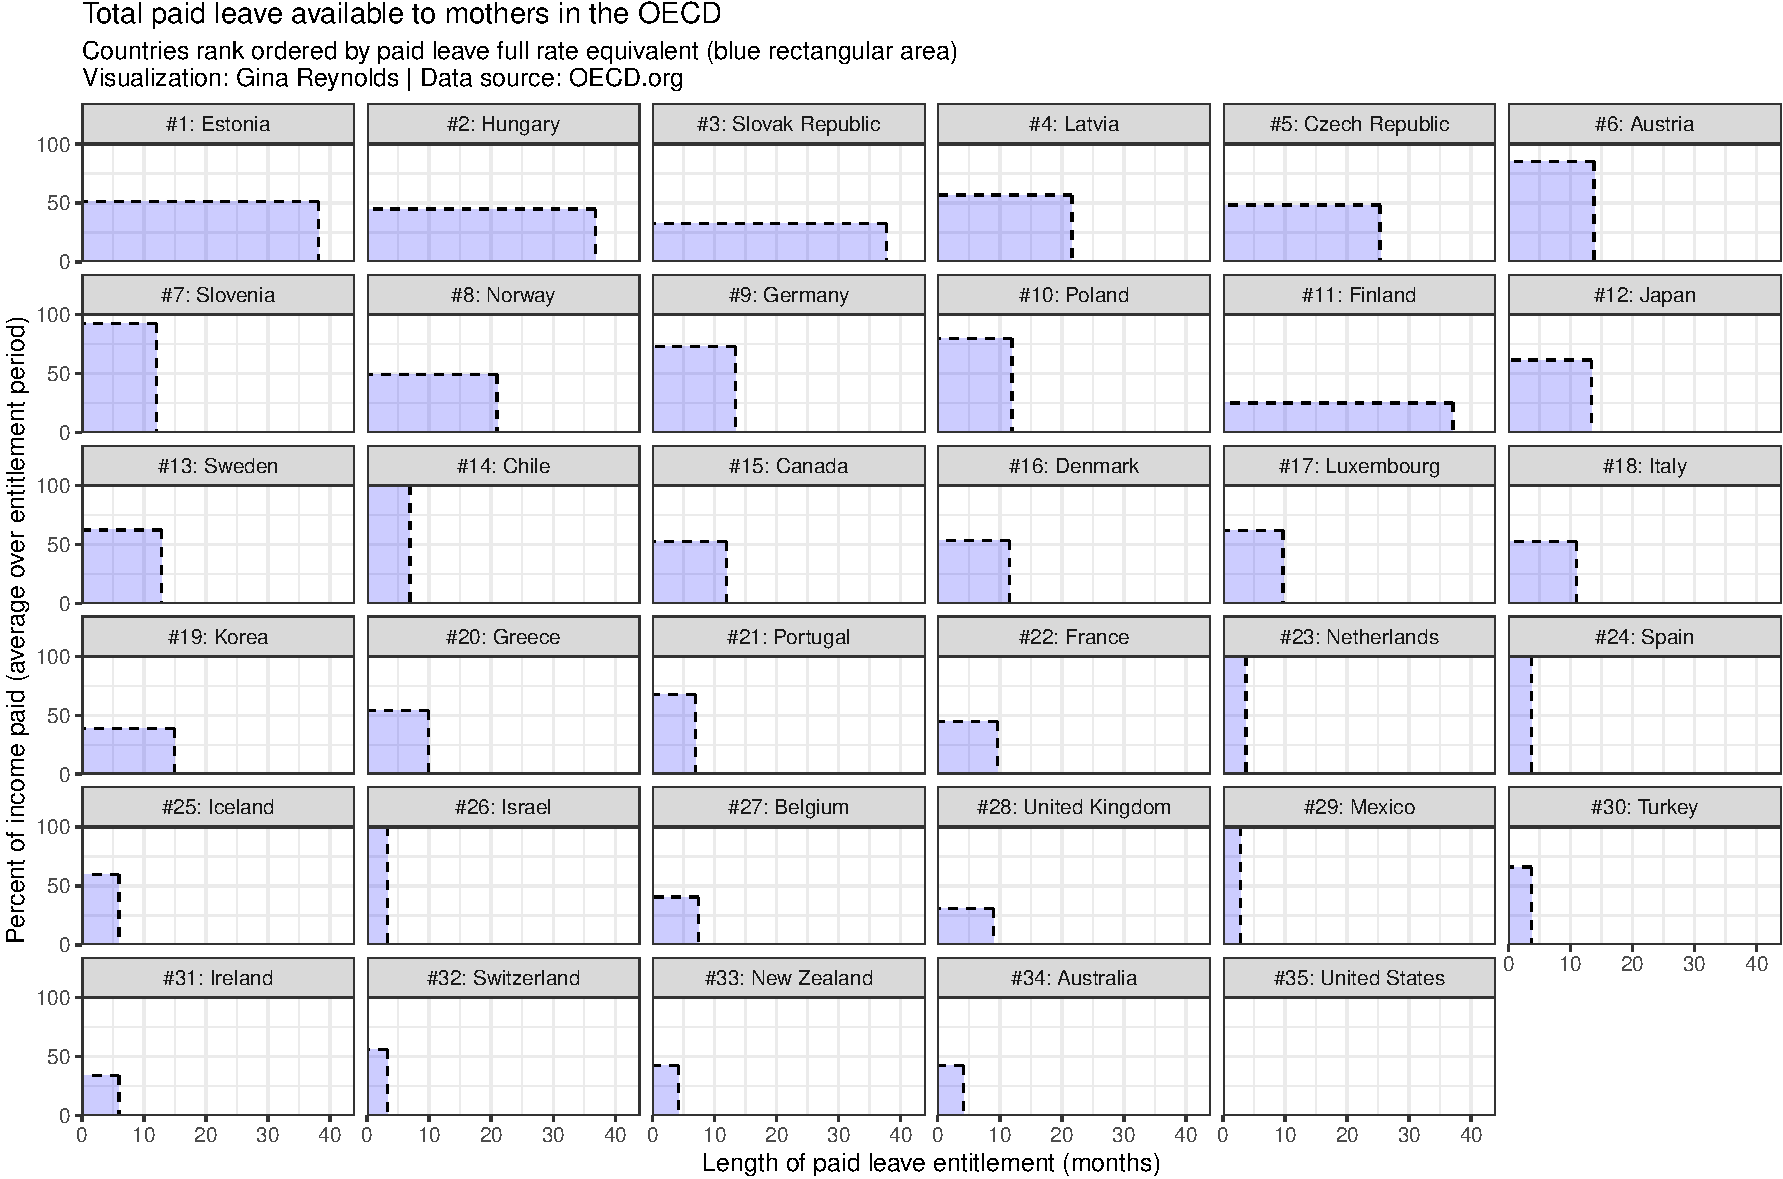
\includegraphics{makeovermonday_book_files/figure-latex/unnamed-chunk-17-1.pdf}

\chapter{Traits}\label{traits}

A random sample from the data set:

\begin{tabular}{l|l|l|r|r|r}
\hline
Gender & Question\_short & Rank (text) & Rank (number) & n & Percent\\
\hline
Men & Money & Ranked first & 1 & 190.78 & 1.787746\\
\hline
Men & Money & Ranked sixth & 6 & 7190.57 & 67.380809\\
\hline
Men & Looks & Ranked fifth & 5 & 2134.35 & 19.967724\\
\hline
Men & Money & Ranked fifth & 5 & 1617.37 & 15.155919\\
\hline
Women & Personality & Ranked fifth & 5 & 608.01 & 5.331190\\
\hline
\end{tabular}

\begin{Shaded}
\begin{Highlighting}[]
\KeywordTok{ggplot}\NormalTok{(}\DataTypeTok{data =}\NormalTok{ world) }\OperatorTok{+}\StringTok{ }
\StringTok{  }\KeywordTok{aes}\NormalTok{(}\DataTypeTok{x =}\NormalTok{ Question_short_wrap) }\OperatorTok{+}
\StringTok{  }\KeywordTok{aes}\NormalTok{(}\DataTypeTok{y =}\NormalTok{ Percent) }\OperatorTok{+}
\StringTok{  }\KeywordTok{aes}\NormalTok{(}\DataTypeTok{fill =} \StringTok{`}\DataTypeTok{Rank (text)}\StringTok{`}\NormalTok{) }\OperatorTok{+}
\StringTok{  }\KeywordTok{facet_grid}\NormalTok{(Gender }\OperatorTok{~}\StringTok{ }\NormalTok{.) }\OperatorTok{+}
\StringTok{  }\KeywordTok{geom_col}\NormalTok{() }\OperatorTok{+}
\StringTok{  }\KeywordTok{coord_flip}\NormalTok{() }\OperatorTok{+}
\StringTok{  }\KeywordTok{scale_fill_manual}\NormalTok{(}
    \DataTypeTok{values =} \KeywordTok{colorRampPalette}\NormalTok{(RColorBrewer}\OperatorTok{::}\KeywordTok{brewer.pal}\NormalTok{(}\DecValTok{9}\NormalTok{, }\StringTok{"Purples"}\NormalTok{))(}\DecValTok{6}\NormalTok{)[}\DecValTok{1}\OperatorTok{:}\DecValTok{6}\NormalTok{],}
    \DataTypeTok{guide =} \KeywordTok{guide_legend}\NormalTok{(}\DataTypeTok{reverse =} \OtherTok{TRUE}\NormalTok{)}
\NormalTok{  ) }\OperatorTok{+}
\StringTok{  }\KeywordTok{labs}\NormalTok{(}\DataTypeTok{fill =} \StringTok{""}\NormalTok{) }\OperatorTok{+}
\StringTok{  }\KeywordTok{xlab}\NormalTok{(}\StringTok{""}\NormalTok{) }\OperatorTok{+}
\StringTok{  }\KeywordTok{labs}\NormalTok{(}\DataTypeTok{title =} \StringTok{"Why do I love thee?  Let me rank the traits... }\CharTok{\textbackslash{}n}\StringTok{How 10,689 men and 11,370 women across 20 countries rank romantic partner trait importance"}\NormalTok{) }\OperatorTok{+}
\StringTok{  }\KeywordTok{labs}\NormalTok{(}\DataTypeTok{subtitle =} \StringTok{"Data Source: @mattsmithetc and @YouGov | Design: Gina Reynolds"}\NormalTok{) }
\end{Highlighting}
\end{Shaded}

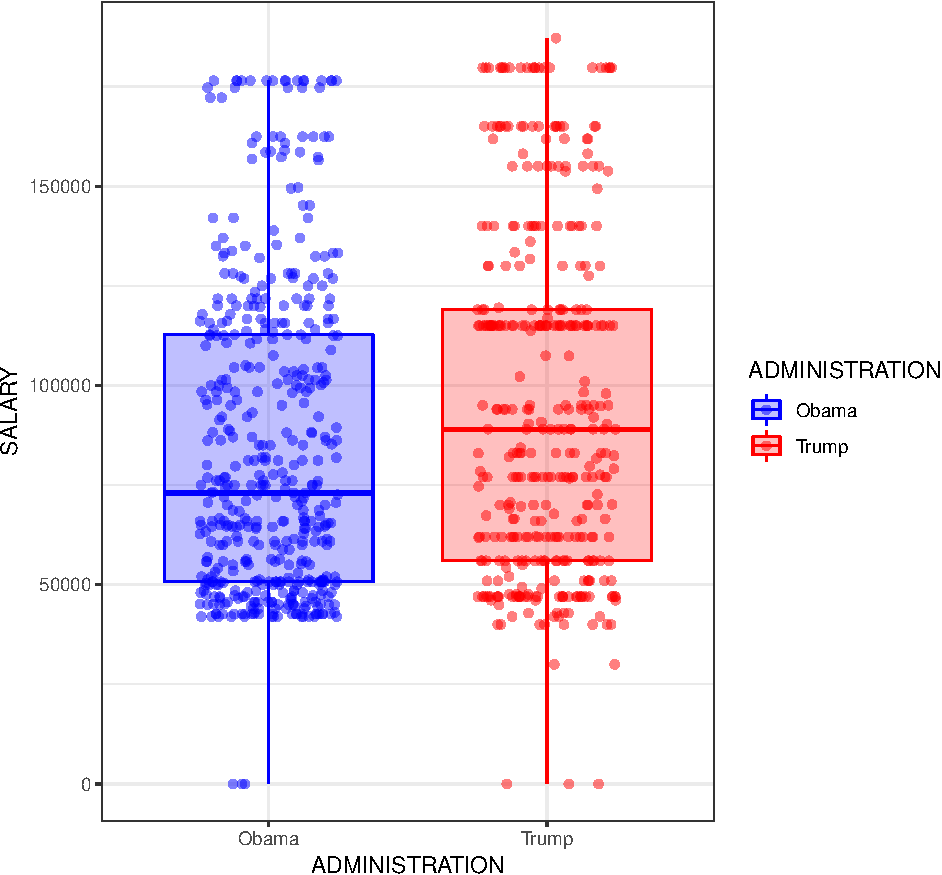
\includegraphics{makeovermonday_book_files/figure-latex/unnamed-chunk-20-1.pdf}

\chapter{Salarys of Trump and Obama White House
Employees}\label{salarys-of-trump-and-obama-white-house-employees}

The data set, originally reported on in an NPR article, shows the
difference in the distribution of salaries for the Obama and early Trump
White House.

First I plot a histogram of each administration. Then I also contrast
boxplots for each administration; the data points are overlayed,
jittered to the widths of the boxplots. Plotly is used to make the graph
interactive; mousing over will allow you to see who the point
represents, their job description and exactly how much they are paid.

A random sample from the data set:

\begin{tabular}{l|l|l|r|l|l}
\hline
ADMINISTRATION & NAME & STATUS & SALARY & PAY BASIS & POSITION TITLE\\
\hline
Obama & Hoover, Zealan T. & Employee & 72000 & Per Annum & POLICY ADVISOR TO THE SENIOR ADVISOR\\
\hline
Trump & Lai, Joseph G. & Employee & 115000 & Per Annum & SPECIAL ASSISTANT TO THE PRESIDENT FOR LEGISLATIVE AFFAIRS\\
\hline
Obama & Dickason, Christine N. & Employee & 42000 & Per Annum & DEPUTY ASSOCIATE DIRECTOR OF CORRESPONDENCE FOR THE FIRST LADY\\
\hline
Obama & Larimer, Becky S. & Employee & 68658 & Per Annum & CALLIGRAPHER\\
\hline
Trump & Salem, Hannah H. & Employee & 83000 & Per Annum & SENIOR LEAD PRESS REPRESENTATIVE\\
\hline
\end{tabular}

\begin{Shaded}
\begin{Highlighting}[]
\KeywordTok{ggplot}\NormalTok{(both_data) }\OperatorTok{+}
\StringTok{  }\KeywordTok{aes}\NormalTok{(}\DataTypeTok{x =}\NormalTok{ ADMINISTRATION) }\OperatorTok{+}\StringTok{ }
\StringTok{  }\KeywordTok{aes}\NormalTok{(}\DataTypeTok{y =}\NormalTok{ SALARY) }\OperatorTok{+}
\StringTok{  }\KeywordTok{geom_jitter}\NormalTok{(}\DataTypeTok{alpha =}\NormalTok{ .}\DecValTok{5}\NormalTok{, }\DataTypeTok{height =} \DecValTok{0}\NormalTok{, }\DataTypeTok{width =}\NormalTok{ .}\DecValTok{25}\NormalTok{) }\OperatorTok{+}
\StringTok{  }\KeywordTok{aes}\NormalTok{(}\DataTypeTok{col =}\NormalTok{ ADMINISTRATION) }\OperatorTok{+}
\StringTok{  }\KeywordTok{geom_boxplot}\NormalTok{(}\DataTypeTok{alpha =}\NormalTok{ .}\DecValTok{25}\NormalTok{) }\OperatorTok{+}
\StringTok{  }\KeywordTok{aes}\NormalTok{(}\DataTypeTok{fill =}\NormalTok{ ADMINISTRATION) }\OperatorTok{+}
\StringTok{  }\KeywordTok{scale_colour_manual}\NormalTok{(}\DataTypeTok{values =} \KeywordTok{c}\NormalTok{(}\StringTok{"blue"}\NormalTok{, }\StringTok{"red"}\NormalTok{)) }\OperatorTok{+}
\StringTok{  }\KeywordTok{scale_fill_manual}\NormalTok{(}\DataTypeTok{values =} \KeywordTok{c}\NormalTok{(}\StringTok{"blue"}\NormalTok{, }\StringTok{"red"}\NormalTok{)) }\OperatorTok{+}
\StringTok{  }\KeywordTok{theme_bw}\NormalTok{()}
\end{Highlighting}
\end{Shaded}

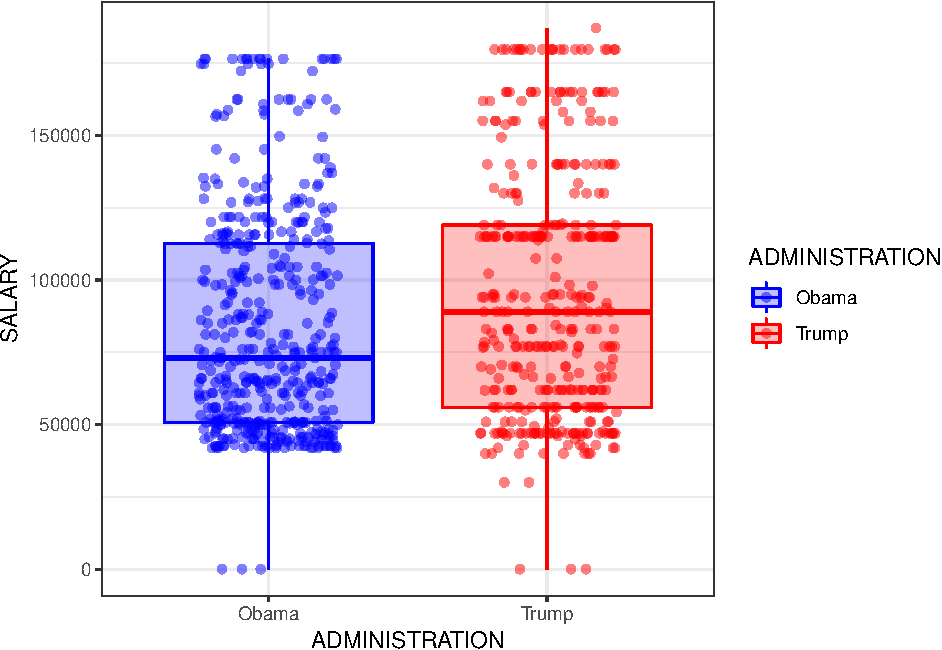
\includegraphics{makeovermonday_book_files/figure-latex/unnamed-chunk-23-1.pdf}

\chapter{Winter Games}\label{winter-games}

A random sample from the data set:

\begin{tabular}{r|l|l|l|l|r|l|l|r}
\hline
Year & Sport & Event & Country & Gender & Medal Rank & Medal & Name of Athlete or Team & Age of Athlete\\
\hline
2006 & Snowboarding & Men's Halfpipe & United States & Men & 2 & silver & Danny Kass & 23\\
\hline
1992 & Alpine Skiing & Men's Combined & Italy & Men & 1 & gold & Josef Polig & 23\\
\hline
2002 & Alpine Skiing & Men's Slalom & France & Men & 2 & silver & Sébastien Amiez & 29\\
\hline
2006 & Cross-Country Skiing & Women's 4 × 5-Kilometer Relay & Germany & Women & 2 & silver & Germany & NA\\
\hline
1956 & Speedskating & Men's 500 Meters & Soviet Union & Men & 2 & silver & Rafael Grach & 23\\
\hline
\end{tabular}

\begin{Shaded}
\begin{Highlighting}[]
\KeywordTok{ggplot}\NormalTok{(}\DataTypeTok{data =}\NormalTok{ dta) }\OperatorTok{+}\StringTok{ }
\StringTok{  }\KeywordTok{aes}\NormalTok{(}\DataTypeTok{x =}\NormalTok{ Year) }\OperatorTok{+}
\StringTok{  }\KeywordTok{aes}\NormalTok{(}\DataTypeTok{y =}\NormalTok{ percent_medals) }\OperatorTok{+}
\StringTok{  }\KeywordTok{geom_line}\NormalTok{() }\OperatorTok{+}\StringTok{ }
\StringTok{  }\KeywordTok{facet_wrap}\NormalTok{(}\OperatorTok{~}\StringTok{ }\NormalTok{Country)}
\end{Highlighting}
\end{Shaded}

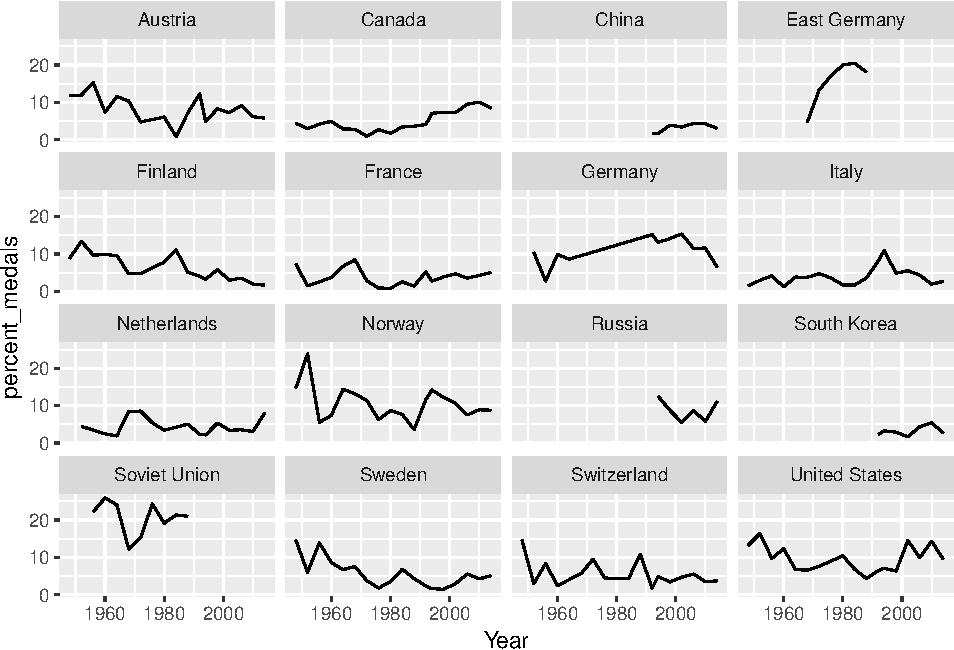
\includegraphics{makeovermonday_book_files/figure-latex/unnamed-chunk-27-1.pdf}

A random sample from the data set:

\begin{tabular}{r|l|l|l|l|r|l|l|r|l}
\hline
Year & Sport & Event & Country & Gender & Medal Rank & Medal & Name of Athlete or Team & Age of Athlete & cold\_war\\
\hline
1994 & Cross-Country Skiing & Men's 30 Kilometers & Norway & Men & 2 & silver & Bjørn Dæhlie & 26 & A\\
\hline
1968 & Cross-Country Skiing & Men's 50 Kilometers & Norway & Men & 1 & gold & Ole Ellefsæter & 28 & A\\
\hline
2006 & Speedskating & Women's 5,000 Meters & Canada & Women & 1 & gold & Clara Hughes & 33 & A\\
\hline
1998 & Ski Jumping & Men's Large Hill, Team & Austria & Men & 3 & bronze & Austria & NA & A\\
\hline
1976 & Speedskating & Men's 1,000 Meters & Norway & Men & 2 & silver & Jørn Didriksen & 22 & A\\
\hline
\end{tabular}

\begin{Shaded}
\begin{Highlighting}[]
\KeywordTok{ggplot}\NormalTok{(dta) }\OperatorTok{+}
\StringTok{  }\KeywordTok{aes}\NormalTok{(}\DataTypeTok{x =}\NormalTok{ Year) }\OperatorTok{+}
\StringTok{  }\KeywordTok{aes}\NormalTok{(}\DataTypeTok{y =} \StringTok{`}\DataTypeTok{Age of Athlete}\StringTok{`}\NormalTok{) }\OperatorTok{+}
\StringTok{  }\KeywordTok{facet_wrap}\NormalTok{(}\OperatorTok{~}\StringTok{ }\NormalTok{Sport, }\DataTypeTok{scales =} \StringTok{"free_y"}\NormalTok{, }\DataTypeTok{nrow =} \DecValTok{2}\NormalTok{) }\OperatorTok{+}
\StringTok{  }\KeywordTok{geom_jitter}\NormalTok{(}\DataTypeTok{size =} \DecValTok{1}\NormalTok{, }\DataTypeTok{mapping =} \KeywordTok{aes}\NormalTok{(}\DataTypeTok{col =} \KeywordTok{fct_inorder}\NormalTok{(Medal))) }\OperatorTok{+}
\StringTok{  }\KeywordTok{geom_smooth}\NormalTok{(}\DataTypeTok{col =} \StringTok{"grey30"}\NormalTok{) }\OperatorTok{+}
\StringTok{  }\KeywordTok{geom_ribbon}\NormalTok{(}\DataTypeTok{ymin =} \DecValTok{20}\NormalTok{, }\DataTypeTok{ymax =} \DecValTok{30}\NormalTok{, }\DataTypeTok{alpha =}\NormalTok{ .}\DecValTok{1}\NormalTok{, }\DataTypeTok{fill =} \StringTok{"blue"}\NormalTok{) }\OperatorTok{+}
\StringTok{  }\KeywordTok{geom_hline}\NormalTok{(}\DataTypeTok{yintercept =} \KeywordTok{c}\NormalTok{(}\DecValTok{20}\NormalTok{, }\DecValTok{30}\NormalTok{), }\DataTypeTok{lty =} \StringTok{"dotted"}\NormalTok{) }\OperatorTok{+}
\StringTok{  }\KeywordTok{geom_hline}\NormalTok{(}\DataTypeTok{yintercept =} \KeywordTok{c}\NormalTok{(}\DecValTok{25}\NormalTok{), }\DataTypeTok{lty =} \StringTok{"dashed"}\NormalTok{) }\OperatorTok{+}
\StringTok{  }\KeywordTok{scale_color_manual}\NormalTok{(}\DataTypeTok{values =} \KeywordTok{c}\NormalTok{(}\StringTok{"goldenrod3"}\NormalTok{, }\StringTok{"grey40"}\NormalTok{, }\StringTok{"goldenrod4"}\NormalTok{), }\DataTypeTok{name =} \StringTok{""}\NormalTok{) }\OperatorTok{+}
\StringTok{  }\KeywordTok{labs}\NormalTok{(}\DataTypeTok{x =} \StringTok{""}\NormalTok{) }\OperatorTok{+}
\StringTok{  }\KeywordTok{labs}\NormalTok{(}\DataTypeTok{title =} \StringTok{"Young and old at the Winter Olympics: medalists' declared ages have risen in recent years"}\NormalTok{) }\OperatorTok{+}\StringTok{ }
\StringTok{  }\KeywordTok{labs}\NormalTok{(}\DataTypeTok{subtitle =} \StringTok{"Includes individual sports that have been in Olympic since 1965"}\NormalTok{) }\OperatorTok{+}
\StringTok{  }\KeywordTok{labs}\NormalTok{(}\DataTypeTok{caption =} \StringTok{"Source: Sports-Reference.com | Vis: Gina Reynolds @EvaMaeRey }\CharTok{\textbackslash{}n}\StringTok{Values 'jittered' to reduce overplotting"}\NormalTok{) }\OperatorTok{+}
\StringTok{  }\KeywordTok{theme_bw}\NormalTok{(}\DataTypeTok{base_size =} \DecValTok{13}\NormalTok{)}
\end{Highlighting}
\end{Shaded}

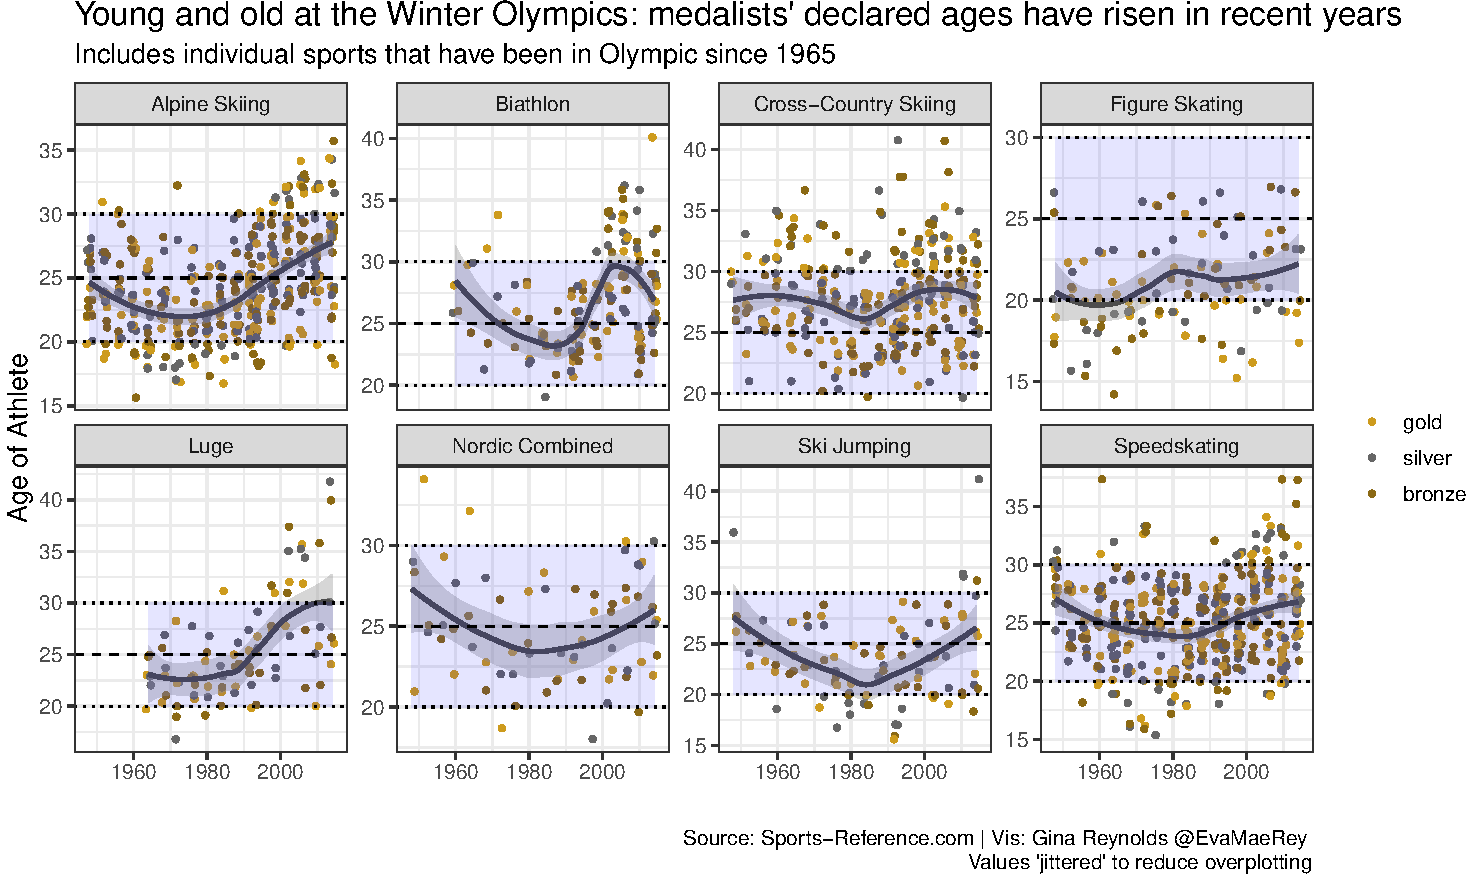
\includegraphics{makeovermonday_book_files/figure-latex/unnamed-chunk-30-1.pdf}

\chapter{Brexit}\label{brexit}

This visualization challenge was a proposed makeover for a Financial
Times visualization focusing on relative economic growth in G7
countries, with an emphasis on growth in the UK, focusing especially
since Brexit. The visualization I present here is not what I created at
the time of the challenge; instead it is inspired by Alan Smith a data
journalist at the Financial Times, who created a really compelling
visualization a couple of months after MakeoverMonday's treatment. I try
to recreate his plot - which uses a ribbon to contain all G7 countries,
and plot the UK's stats thereover. This declutters the graph, and makes
you focus on where the UK falls among other countries, without being
needlessly specific about those countries; the data story isn't about
them anyway, might be Smith's thinking. My graph actually lightly traces
economic growth in other countries, but deemphasizes their importance,
like Smith.

A random sample from the data set:

\begin{tabular}{l|r|r|l|r|l}
\hline
Country & Year & Quarter & Date (start of quarter) & Percentage change from previous period & Date (start o quarter)\\
\hline
GBR & 2013 & 4 & 2013-10-01 & 0.491800 & 2013-10-01\\
\hline
ITA & 2012 & 2 & 2012-04-01 & -0.790043 & 2012-04-01\\
\hline
USA & 2015 & 4 & 2015-10-01 & 0.121010 & 2015-10-01\\
\hline
ITA & 2013 & 4 & 2013-10-01 & -0.039854 & 2013-10-01\\
\hline
GBR & 2010 & 1 & 2010-01-01 & 0.549599 & 2010-01-01\\
\hline
\end{tabular}

\begin{Shaded}
\begin{Highlighting}[]
\KeywordTok{ggplot}\NormalTok{(}\DataTypeTok{data =}\NormalTok{ data) }\OperatorTok{+}
\StringTok{  }\KeywordTok{aes}\NormalTok{(}\DataTypeTok{x =} \StringTok{`}\DataTypeTok{Date (start of quarter)}\StringTok{`}\NormalTok{) }\OperatorTok{+}
\StringTok{  }\KeywordTok{aes}\NormalTok{(}\DataTypeTok{y =} \StringTok{`}\DataTypeTok{Percentage change from previous period}\StringTok{`}\NormalTok{) }\OperatorTok{+}
\StringTok{  }\KeywordTok{facet_wrap}\NormalTok{(}\OperatorTok{~}\StringTok{ }\NormalTok{Country) }\OperatorTok{+}
\StringTok{  }\KeywordTok{geom_line}\NormalTok{() }\OperatorTok{+}
\StringTok{  }\KeywordTok{geom_hline}\NormalTok{(}\DataTypeTok{yintercept =} \DecValTok{0}\NormalTok{, }\DataTypeTok{col =} \StringTok{"grey"}\NormalTok{) }\OperatorTok{+}
\StringTok{  }\KeywordTok{geom_vline}\NormalTok{(}\DataTypeTok{xintercept =} \KeywordTok{as.numeric}\NormalTok{(}\KeywordTok{as.POSIXct}\NormalTok{(}\StringTok{"2016-06-23"}\NormalTok{)), }\DataTypeTok{lty =} \StringTok{"dashed"}\NormalTok{) }\OperatorTok{+}
\StringTok{  }\KeywordTok{labs}\NormalTok{(}\DataTypeTok{title =} \StringTok{"Quarterly GDP Growth in Relation to Brexit Vote"}\NormalTok{) }\OperatorTok{+}
\StringTok{  }\KeywordTok{labs}\NormalTok{(}\DataTypeTok{subtitle =} \StringTok{"Source: OECD"}\NormalTok{)}
\end{Highlighting}
\end{Shaded}

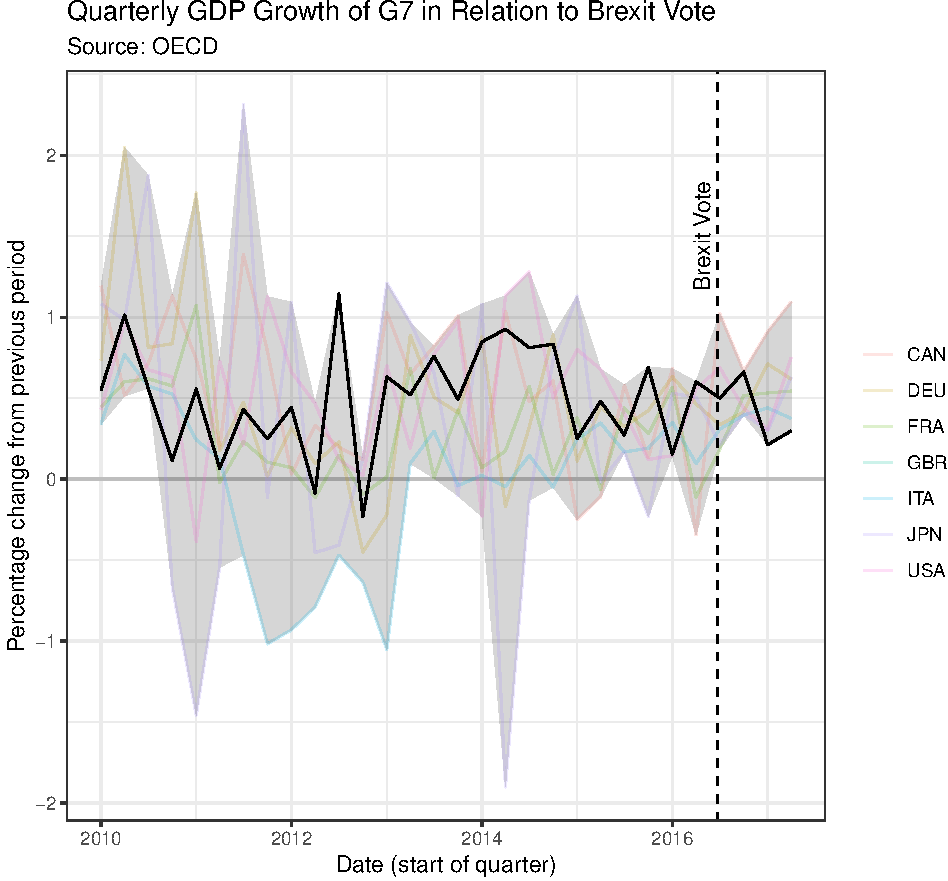
\includegraphics{makeovermonday_book_files/figure-latex/unnamed-chunk-33-1.pdf}

A random sample from the data set:

\begin{tabular}{l|r|r|l|r|l|r|r}
\hline
Country & Year & Quarter & Date (start of quarter) & Percentage change from previous period & Date (start o quarter) & min\_ & max\_\\
\hline
DEU & 2011 & 3 & 2011-07-01 & 0.474351 & 2011-07-01 & -0.468615 & 2.312151\\
\hline
CAN & 2013 & 4 & 2013-10-01 & 1.007924 & 2013-10-01 & -0.102503 & 1.007924\\
\hline
ITA & 2016 & 3 & 2016-07-01 & 0.308248 & 2016-07-01 & 0.185529 & 1.021803\\
\hline
DEU & 2013 & 2 & 2013-04-01 & 0.886494 & 2013-04-01 & 0.096773 & 0.967565\\
\hline
FRA & 2016 & 2 & 2016-04-01 & -0.112590 & 2016-04-01 & -0.343549 & 0.601298\\
\hline
\end{tabular}

\begin{Shaded}
\begin{Highlighting}[]
\KeywordTok{ggplot}\NormalTok{(}\DataTypeTok{data =}\NormalTok{ data) }\OperatorTok{+}
\StringTok{  }\KeywordTok{aes}\NormalTok{(}\DataTypeTok{x =} \StringTok{`}\DataTypeTok{Date (start of quarter)}\StringTok{`}\NormalTok{) }\OperatorTok{+}
\StringTok{  }\KeywordTok{aes}\NormalTok{(}\DataTypeTok{y =} \StringTok{`}\DataTypeTok{Percentage change from previous period}\StringTok{`}\NormalTok{) }\OperatorTok{+}
\StringTok{  }\KeywordTok{aes}\NormalTok{(}\DataTypeTok{ymin =}\NormalTok{ min_) }\OperatorTok{+}
\StringTok{  }\KeywordTok{aes}\NormalTok{(}\DataTypeTok{ymax =}\NormalTok{ max_) }\OperatorTok{+}
\StringTok{  }\KeywordTok{geom_hline}\NormalTok{(}\DataTypeTok{yintercept =} \DecValTok{0}\NormalTok{, }\DataTypeTok{col =} \StringTok{"grey"}\NormalTok{) }\OperatorTok{+}
\StringTok{  }\KeywordTok{geom_ribbon}\NormalTok{(}\DataTypeTok{alpha =}\NormalTok{ .}\DecValTok{2}\NormalTok{) }\OperatorTok{+}
\StringTok{  }\KeywordTok{geom_line}\NormalTok{(}\KeywordTok{aes}\NormalTok{(}\DataTypeTok{col =}\NormalTok{ Country), }\DataTypeTok{alpha =}\NormalTok{ .}\DecValTok{2}\NormalTok{) }\OperatorTok{+}
\StringTok{  }\KeywordTok{geom_line}\NormalTok{(}\DataTypeTok{data =}\NormalTok{ data }\OperatorTok\StringTok{ }\KeywordTok{filter}\NormalTok{(Country }\OperatorTok{==}\StringTok{ "GBR"}\NormalTok{), }\DataTypeTok{col =} \StringTok{"black"}\NormalTok{) }\OperatorTok{+}
\StringTok{  }\KeywordTok{geom_vline}\NormalTok{(}\DataTypeTok{xintercept =} \KeywordTok{as.numeric}\NormalTok{(}\KeywordTok{as.POSIXct}\NormalTok{(}\StringTok{"2016-06-23"}\NormalTok{)), }\DataTypeTok{lty =} \DecValTok{2}\NormalTok{) }\OperatorTok{+}
\StringTok{  }\KeywordTok{annotate}\NormalTok{(}
    \DataTypeTok{geom =} \StringTok{"text"}\NormalTok{, }\DataTypeTok{x =} \KeywordTok{as.POSIXct}\NormalTok{(}\StringTok{"2016-04-23"}\NormalTok{), }\DataTypeTok{y =} \FloatTok{1.5}\NormalTok{,}
    \DataTypeTok{label =} \StringTok{"Brexit Vote"}\NormalTok{, }\DataTypeTok{angle =} \DecValTok{90}
\NormalTok{  ) }\OperatorTok{+}
\StringTok{  }\KeywordTok{labs}\NormalTok{(}
    \DataTypeTok{title =} \StringTok{"Quarterly GDP Growth of G7 in Relation to Brexit Vote"}\NormalTok{,}
    \DataTypeTok{subtitle =} \StringTok{"Source: OECD"}\NormalTok{,}
    \DataTypeTok{col =} \StringTok{""}
\NormalTok{  ) }\OperatorTok{+}
\StringTok{  }\KeywordTok{theme_bw}\NormalTok{()}
\end{Highlighting}
\end{Shaded}

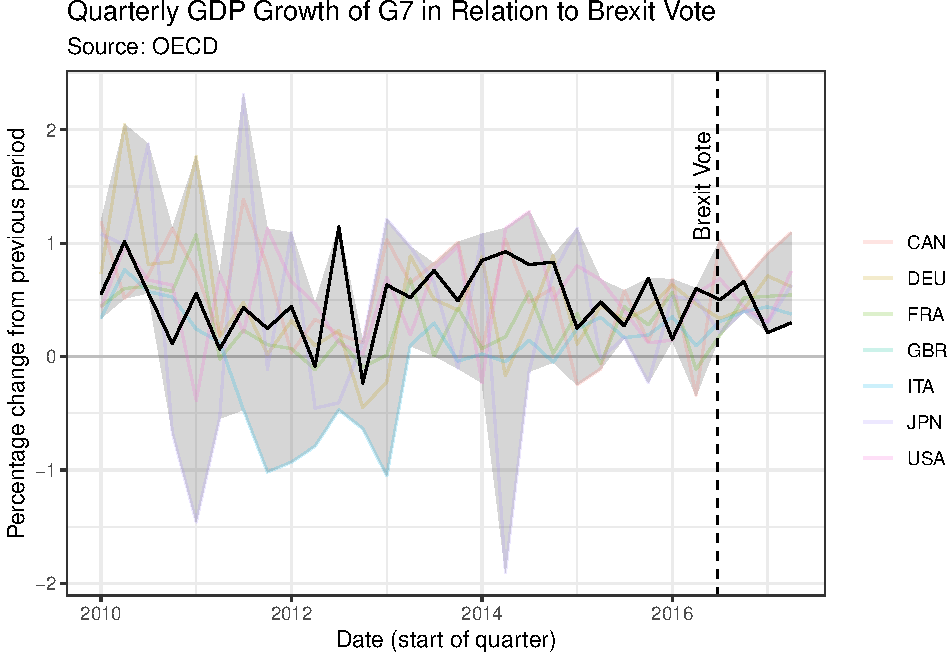
\includegraphics{makeovermonday_book_files/figure-latex/unnamed-chunk-36-1.pdf}

\chapter{Curry in London}\label{curry-in-london}

This visualization task seemed to get at the question: Does where you
eat matter. The data was the cost of identical menu items at different
locations of the same restaurant, the Wetherspoon, around the UK.

First, I mapped the cost of a single menu item, the Empire Burger,
across the UK. Then, I calculated the distance from Wetherspoon
restaurants from the Big Ben, and plotted prices as a function of this
distance -- plotting only the restaurants in a 10 kilometer radius.

A random sample from the data set:

\begin{tabular}{l|l|r|r|r|r|r|r|r|r|r|r|r|l|r|r|l|r|r}
\hline
Name & Location & Latitude & Longitude & Empire State Burger & Chicken Tikka & Gammon afternoon deal & Chocolate Brownie & Doom Bar & Birra Moretti & Porn Star at 2 x £12 & Porn Star (glass) & MEAL & Notes & Moretti as a \% of a tikka & Moretti as \% of burger & PRICE BUCKETS & Food cost £ & Drink cost £\\
\hline
The Moon Under Water & Milton Keynes & 52.04181 & -0.7488899 & 8.75 & 7.49 & 5.90 & 3.85 & 2.25 & 3.15 & 6.3 & NA & 25.49 & NA & 0.4205607 & 0.3600000 & £25.21+ & 16.24 & 5.40\\
\hline
The Observatory & Ilkeston & 52.97154 & -1.3081310 & 8.75 & 6.99 & 5.90 & 3.85 & 2.29 & 2.99 & 6.3 & NA & 24.87 & NA & 0.4277539 & 0.3417143 & £25.20- & 15.74 & 5.28\\
\hline
The Counting House & Congleton & 53.16386 & -2.2146526 & 8.75 & 7.40 & 5.90 & 3.85 & 2.29 & 3.09 & 6.3 & NA & 25.38 & NA & 0.4175676 & 0.3531429 & £25.21+ & 16.15 & 5.38\\
\hline
The Christopher Creeke & Bournemouth & 50.72238 & -1.8657451 & 8.75 & 6.40 & 5.99 & 3.40 & 2.29 & 3.19 & 6.3 & NA & 24.03 & NA & 0.4984375 & 0.3645714 & £25.20- & 15.15 & 5.48\\
\hline
Bull and Stirrup Hotel & Chester & 53.19436 & -2.8933313 & 9.10 & 7.79 & 6.40 & 3.85 & 2.59 & 3.25 & 6.3 & NA & 26.58 & NA & 0.4172015 & 0.3571429 & £25.21+ & 16.89 & 5.84\\
\hline
\end{tabular}

\begin{Shaded}
\begin{Highlighting}[]
\CommentTok{# Mapping data}
\NormalTok{world_map_df <-}\StringTok{ }\KeywordTok{map_data}\NormalTok{(}\StringTok{"world"}\NormalTok{)}
\end{Highlighting}
\end{Shaded}

A random sample from the data set:

\begin{tabular}{l|r|r|r|r|l|l}
\hline
  & long & lat & group & order & region & subregion\\
\hline
71407 & -72.28902 & -9.629199 & 1124 & 71407 & Peru & NA\\
\hline
89141 & 54.47285 & 42.180176 & 1418 & 89141 & Turkmenistan & NA\\
\hline
100607 & 27.57383 & -12.227051 & 1623 & 100607 & Zambia & NA\\
\hline
34107 & -81.81622 & 22.200195 & 457 & 34107 & Cuba & NA\\
\hline
82254 & 138.66074 & 53.744774 & 1309 & 82254 & Russia & NA\\
\hline
\end{tabular}

\begin{Shaded}
\begin{Highlighting}[]
\CommentTok{# create a blank ggplot theme}
\NormalTok{theme_opts <-}\StringTok{ }\KeywordTok{theme}\NormalTok{(}
  \DataTypeTok{panel.grid.minor =} \KeywordTok{element_blank}\NormalTok{(),}
  \DataTypeTok{panel.grid.major =} \KeywordTok{element_blank}\NormalTok{(),}
  \DataTypeTok{panel.background =} \KeywordTok{element_blank}\NormalTok{(),}
  \DataTypeTok{plot.background =} \KeywordTok{element_rect}\NormalTok{(}\DataTypeTok{fill =} \StringTok{"#e6e8ed"}\NormalTok{),}
  \DataTypeTok{panel.border =} \KeywordTok{element_blank}\NormalTok{(),}
  \DataTypeTok{axis.line =} \KeywordTok{element_blank}\NormalTok{(),}
  \DataTypeTok{axis.text.x =} \KeywordTok{element_blank}\NormalTok{(),}
  \DataTypeTok{axis.text.y =} \KeywordTok{element_blank}\NormalTok{(),}
  \DataTypeTok{axis.ticks =} \KeywordTok{element_blank}\NormalTok{(),}
  \DataTypeTok{axis.title.x =} \KeywordTok{element_blank}\NormalTok{(),}
  \DataTypeTok{axis.title.y =} \KeywordTok{element_blank}\NormalTok{(),}
  \DataTypeTok{plot.title =} \KeywordTok{element_text}\NormalTok{(}\DataTypeTok{size =} \DecValTok{15}\NormalTok{)}
\NormalTok{)}


\KeywordTok{ggplot}\NormalTok{(}\DataTypeTok{data =}\NormalTok{ world_map_df }\OperatorTok\StringTok{ }\KeywordTok{filter}\NormalTok{(region }\OperatorTok{==}\StringTok{ "UK"}\NormalTok{)) }\OperatorTok{+}
\StringTok{  }\KeywordTok{aes}\NormalTok{(}\DataTypeTok{x =}\NormalTok{ long) }\OperatorTok{+}
\StringTok{  }\KeywordTok{aes}\NormalTok{(}\DataTypeTok{y =}\NormalTok{ lat) }\OperatorTok{+}
\StringTok{  }\KeywordTok{aes}\NormalTok{(}\DataTypeTok{group =}\NormalTok{ group) }\OperatorTok{+}
\StringTok{  }\KeywordTok{geom_polygon}\NormalTok{(}\DataTypeTok{fill =} \StringTok{"white"}\NormalTok{) }\OperatorTok{+}
\StringTok{  }\KeywordTok{coord_equal}\NormalTok{() }\OperatorTok{+}
\StringTok{  }\KeywordTok{scale_fill_viridis_c}\NormalTok{(}\DataTypeTok{option =} \StringTok{"viridis"}\NormalTok{) }\OperatorTok{+}
\StringTok{  }\KeywordTok{geom_point}\NormalTok{(}\DataTypeTok{data =}\NormalTok{ data0,}
             \DataTypeTok{mapping =} \KeywordTok{aes}\NormalTok{(}\DataTypeTok{x =}\NormalTok{ Longitude, }\DataTypeTok{y =}\NormalTok{ Latitude,}
                           \DataTypeTok{group =} \OtherTok{NULL}\NormalTok{, }\DataTypeTok{fill =} \StringTok{`}\DataTypeTok{Empire State Burger}\StringTok{`}\NormalTok{),}
    \DataTypeTok{colour =} \StringTok{"black"}\NormalTok{, }\DataTypeTok{shape =} \DecValTok{21}\NormalTok{, }\DataTypeTok{stroke =} \DecValTok{1}\NormalTok{, }\DataTypeTok{alpha =}\NormalTok{ .}\DecValTok{5}\NormalTok{, }\DataTypeTok{size =} \DecValTok{3}
\NormalTok{  ) }\OperatorTok{+}
\StringTok{  }\KeywordTok{labs}\NormalTok{(}\DataTypeTok{fill =} \StringTok{"Price}\CharTok{\textbackslash{}n}\StringTok{(Pounds)"}\NormalTok{) }\OperatorTok{+}
\StringTok{  }\KeywordTok{labs}\NormalTok{(}\DataTypeTok{title =} \StringTok{"Empire State Burger Price"}\NormalTok{) }\OperatorTok{+}
\StringTok{  }\KeywordTok{labs}\NormalTok{(}\DataTypeTok{subtitle =} \StringTok{"@EvaMaeRey | source: data.worldbank.org"}\NormalTok{) }\OperatorTok{+}
\StringTok{  }\NormalTok{theme_opts }
\end{Highlighting}
\end{Shaded}

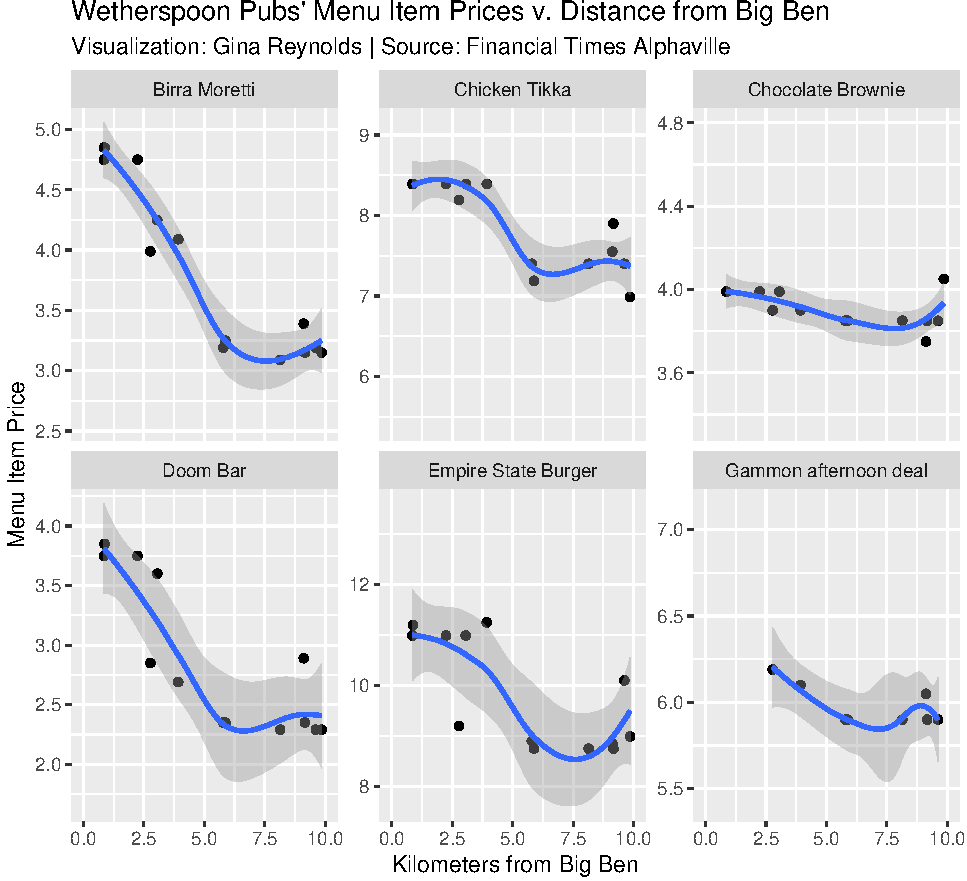
\includegraphics{makeovermonday_book_files/figure-latex/unnamed-chunk-41-1.pdf}

A random sample from the data set:

\begin{tabular}{l|l|r|r|l|r|r|l|r|r|r|l|r}
\hline
Name & Location & Latitude & Longitude & Notes & Moretti as a \% of a tikka & Moretti as \% of burger & PRICE BUCKETS & Food cost £ & Drink cost £ & Kilometers from Big Ben & Item & Menu Item Price\\
\hline
The Muckle Cross & Elgin & 57.64887 & -3.3124440 & NA & 0.3770270 & 0.3188571 & £25.20- & 16.15 & 4.74 & 713.66817 & Chicken Tikka & 7.40\\
\hline
The Hatchet Inn & Newbury & 51.40082 & -1.3228789 & NA & 0.4581081 & 0.3874286 & £25.21+ & 16.15 & 5.88 & 84.71407 & Birra Moretti & 3.39\\
\hline
The Smithy Fold & Glossop & 53.44258 & -1.9487549 & NA & 0.4175676 & 0.3551724 & £25.21+ & 16.10 & 5.58 & 248.42319 & Gammon afternoon deal & 5.85\\
\hline
The Robert Peel & Bury & 53.59381 & -2.2981393 & NA & 0.4297636 & 0.3531429 & £25.20- & 15.94 & 5.38 & 275.00341 & Chocolate Brownie & 3.85\\
\hline
The Coliseum Picture Theatre & Cleethorpes & 53.56090 & -0.0312133 & NA & 0.4018445 & 0.3485714 & £25.21+ & 16.34 & 5.34 & 228.25354 & Gammon afternoon deal & 5.90\\
\hline
\end{tabular}

\begin{Shaded}
\begin{Highlighting}[]
\KeywordTok{ggplot}\NormalTok{(}\DataTypeTok{data =}\NormalTok{ dataLong) }\OperatorTok{+}
\StringTok{  }\KeywordTok{aes}\NormalTok{(}\DataTypeTok{x =} \StringTok{`}\DataTypeTok{Kilometers from Big Ben}\StringTok{`}\NormalTok{) }\OperatorTok{+}
\StringTok{  }\KeywordTok{aes}\NormalTok{(}\DataTypeTok{y =} \StringTok{`}\DataTypeTok{Menu Item Price}\StringTok{`}\NormalTok{) }\OperatorTok{+}
\StringTok{  }\KeywordTok{facet_wrap}\NormalTok{(}\OperatorTok{~}\StringTok{ }\NormalTok{Item, }\DataTypeTok{scales =} \StringTok{"free_y"}\NormalTok{) }\OperatorTok{+}
\StringTok{  }\KeywordTok{geom_point}\NormalTok{() }\OperatorTok{+}
\StringTok{  }\KeywordTok{geom_smooth}\NormalTok{() }\OperatorTok{+}
\StringTok{  }\KeywordTok{xlim}\NormalTok{(}\KeywordTok{c}\NormalTok{(}\DecValTok{0}\NormalTok{, }\DecValTok{10}\NormalTok{)) }\OperatorTok{+}
\StringTok{  }\KeywordTok{labs}\NormalTok{(}\DataTypeTok{title =} \StringTok{"Wetherspoon Pubs' Menu Item Prices v. Distance from Big Ben"}\NormalTok{) }\OperatorTok{+}
\StringTok{  }\KeywordTok{labs}\NormalTok{(}\DataTypeTok{subtitle =} \StringTok{"Visualization: Gina Reynolds | Source: Financial Times Alphaville"}\NormalTok{) }
\end{Highlighting}
\end{Shaded}

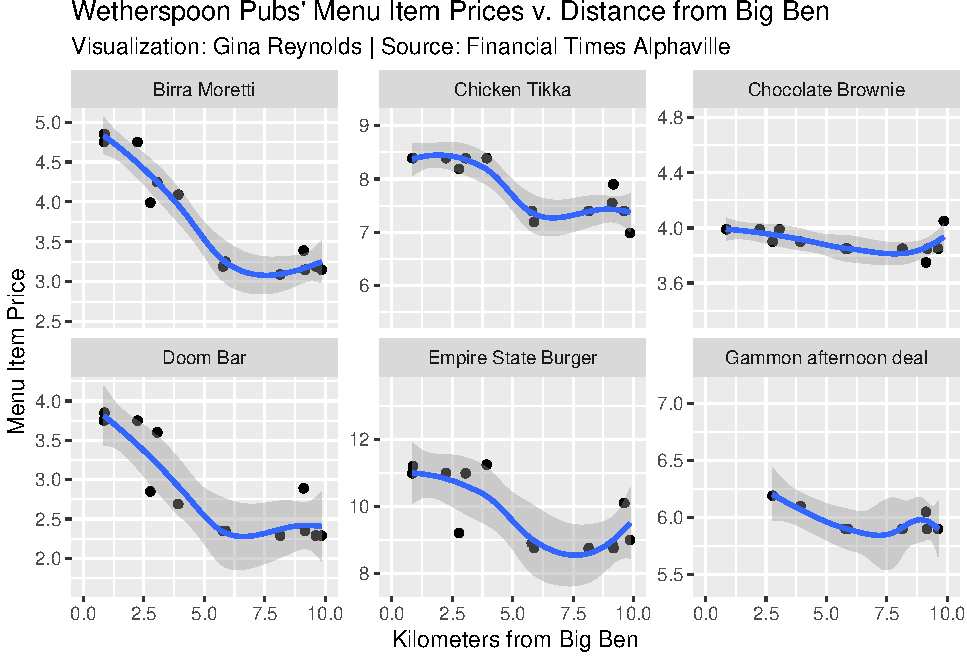
\includegraphics{makeovermonday_book_files/figure-latex/unnamed-chunk-44-1.pdf}

\chapter{Life Expectancy Increases}\label{life-expectancy-increases}

To dramatically show the increases in life expectancy by country from
1960 to 2010, I plot the variable in 1960 versus itself in 2010. The
line of equivilance (a 45\% angle) is used as a reference and shows the
result that you would see if there where no growth. The vertical
distance from this line is the increase in life expectancy. I also
superimpose a linear model on top of the scatter plot. You can see that
the gains are greater for countries that started off with lower life
expectancies.

A random sample from the data set:

\begin{tabular}{r|l|l|l|l|r|r|l|r}
\hline
Life Expectancy 1960 & Country Code & Country Name & Region & Income Group & Year & Life Expectancy 2010 & CountryName & squared\\
\hline
73.42317 & ISL & Iceland & Europe \& Central Asia & High income & 2010 & 81.89756 & Iceland & 5390.962\\
\hline
58.69405 & UZB & Uzbekistan & Europe \& Central Asia & Lower middle income & 2010 & 69.96844 & Uzbekistan & 3444.991\\
\hline
62.72905 & BHS & Bahamas, The & Latin America \& Caribbean & High income & 2010 & 74.59690 & Bahamas & 3934.934\\
\hline
59.73227 & LKA & Sri Lanka & South Asia & Lower middle income & 2010 & 74.31302 & Sri Lanka & 3567.944\\
\hline
41.01805 & COD & Congo, Dem. Rep. & Sub-Saharan Africa & Low income & 2010 & 56.87017 & Congo - Kinshasa & 1682.480\\
\hline
\end{tabular}

\begin{Shaded}
\begin{Highlighting}[]
\KeywordTok{ggplot}\NormalTok{(compare) }\OperatorTok{+}
\StringTok{  }\KeywordTok{aes}\NormalTok{(}\DataTypeTok{x =} \StringTok{`}\DataTypeTok{Life Expectancy 1960}\StringTok{`}\NormalTok{) }\OperatorTok{+}\StringTok{ }
\StringTok{  }\KeywordTok{aes}\NormalTok{(}\DataTypeTok{y =} \StringTok{`}\DataTypeTok{Life Expectancy 2010}\StringTok{`}\NormalTok{) }\OperatorTok{+}
\StringTok{  }\KeywordTok{geom_point}\NormalTok{() }\OperatorTok{+}
\StringTok{  }\KeywordTok{geom_smooth}\NormalTok{(}\DataTypeTok{se =}\NormalTok{ F, }\DataTypeTok{method =} \StringTok{"lm"}\NormalTok{) }\OperatorTok{+}
\StringTok{  }\KeywordTok{geom_abline}\NormalTok{(}\DataTypeTok{slope =} \DecValTok{1}\NormalTok{, }\DataTypeTok{intercept =} \DecValTok{0}\NormalTok{, }\DataTypeTok{lty =} \DecValTok{2}\NormalTok{) }\OperatorTok{+}
\StringTok{  }\CommentTok{# coord_fixed() +}
\StringTok{  }\KeywordTok{aes}\NormalTok{(}\DataTypeTok{xend =} \StringTok{`}\DataTypeTok{Life Expectancy 1960}\StringTok{`}\NormalTok{) }\OperatorTok{+}
\StringTok{  }\KeywordTok{aes}\NormalTok{(}\DataTypeTok{yend =} \StringTok{`}\DataTypeTok{Life Expectancy 1960}\StringTok{`}\NormalTok{) }\OperatorTok{+}
\StringTok{  }\KeywordTok{geom_segment}\NormalTok{(}\DataTypeTok{mapping =} \KeywordTok{aes}\NormalTok{(}\DataTypeTok{col =} \StringTok{"Gain from 1960 to 2010"}\NormalTok{)) }\OperatorTok{+}
\StringTok{  }\KeywordTok{geom_segment}\NormalTok{(}\DataTypeTok{mapping =} \KeywordTok{aes}\NormalTok{(}\DataTypeTok{y =} \DecValTok{0}\NormalTok{, }\DataTypeTok{col =} \StringTok{"Country Expectancy in 1960"}\NormalTok{)) }\OperatorTok{+}
\StringTok{  }\KeywordTok{scale_color_manual}\NormalTok{(}
    \DataTypeTok{breaks =} \KeywordTok{c}\NormalTok{(}
      \StringTok{"Gain from 1960 to 2010"}\NormalTok{,}
      \StringTok{"Country Expectancy in 1960"}
\NormalTok{    ),}
    \DataTypeTok{values =} \KeywordTok{c}\NormalTok{(}\StringTok{"grey59"}\NormalTok{, }\StringTok{"grey30"}\NormalTok{, }\StringTok{"grey30"}\NormalTok{)}
\NormalTok{  ) }\OperatorTok{+}
\StringTok{  }\KeywordTok{geom_point}\NormalTok{(}\KeywordTok{aes}\NormalTok{(}\DataTypeTok{y =} \StringTok{`}\DataTypeTok{Life Expectancy 1960}\StringTok{`}\NormalTok{), }\DataTypeTok{col =} \StringTok{"grey30"}\NormalTok{) }\OperatorTok{+}
\StringTok{  }\KeywordTok{geom_point}\NormalTok{() }\OperatorTok{+}
\StringTok{  }\KeywordTok{labs}\NormalTok{(}\DataTypeTok{subtitle =} \StringTok{"@EvaMaeRey | source: data.worldbank.org"}\NormalTok{, }\DataTypeTok{size =}\NormalTok{ .}\DecValTok{7}\NormalTok{) }\OperatorTok{+}
\StringTok{  }\KeywordTok{labs}\NormalTok{(}\DataTypeTok{title =} \StringTok{"Life Expectancy at Birth by Country"}\NormalTok{) }\OperatorTok{+}\StringTok{ }
\StringTok{  }\KeywordTok{labs}\NormalTok{(}\DataTypeTok{col =} \StringTok{""}\NormalTok{) }\OperatorTok{+}
\StringTok{  }\KeywordTok{theme}\NormalTok{(}\DataTypeTok{legend.title =} \KeywordTok{element_blank}\NormalTok{()) }\OperatorTok{+}
\StringTok{  }\KeywordTok{theme_bw}\NormalTok{() }\OperatorTok{+}
\StringTok{  }\KeywordTok{xlim}\NormalTok{(}\KeywordTok{c}\NormalTok{(}\DecValTok{20}\NormalTok{, }\DecValTok{80}\NormalTok{))}
\end{Highlighting}
\end{Shaded}

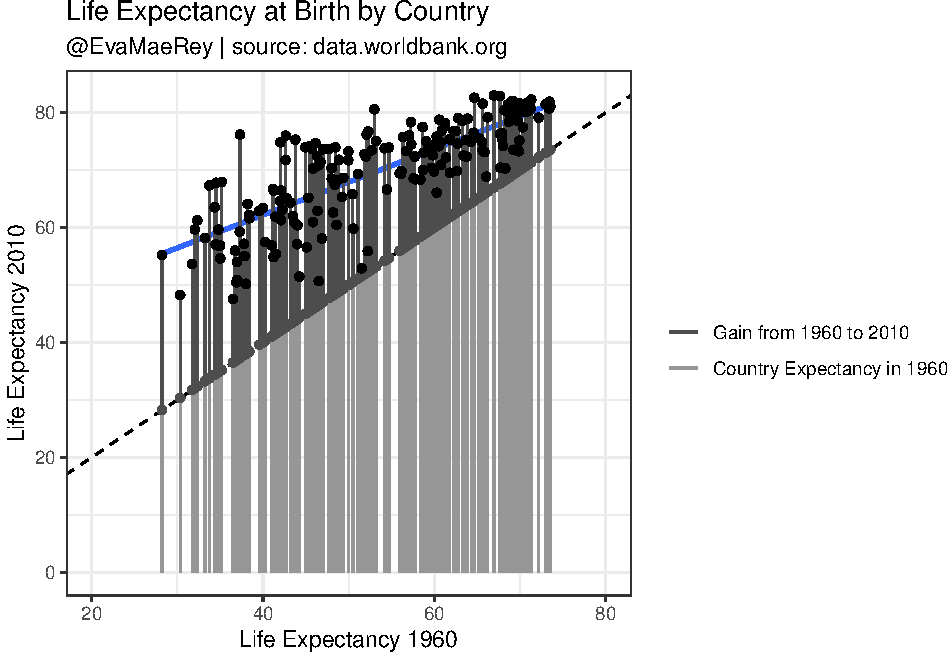
\includegraphics{makeovermonday_book_files/figure-latex/unnamed-chunk-47-1.pdf}

\chapter{Myers Briggs}\label{myers-briggs}

This data looks at the relationship betweeen four binary variables. The
challenge is how to display that in one visualization. My first idea was
to use a mosaic plot. However, I came across advice from ``The
Perceptual Edge'', that generally advised against the use of the mosaic
plot, instead favoring a kind of nested bar plot. I tried to implement
that. While I do think that it is pretty, I think that it still requires
a lot of the reader to interpret the graph. Perhaps more annotation
could alleviate this burden.

A random sample from the data set:

\begin{tabular}{l|l|l|l|r}
\hline
(S)ensing/I(N)tuition & (T)hinking/(F)eeling & (J)udging/(P)erceiving & (E)xtroversion/(I)ntroversion & count\\
\hline
Sensing & Thinking & Judging & Introversion & 1\\
\hline
Sensing & Thinking & Perceiving & Introversion & 1\\
\hline
Sensing & Thinking & Judging & Introversion & 1\\
\hline
Sensing & Feeling & Perceiving & Extroversion & 1\\
\hline
Intuition & Thinking & Perceiving & Introversion & 1\\
\hline
\end{tabular}

\begin{Shaded}
\begin{Highlighting}[]
\KeywordTok{ggplot}\NormalTok{(d) }\OperatorTok{+}
\StringTok{  }\KeywordTok{aes}\NormalTok{(}\DataTypeTok{x =} \StringTok{`}\DataTypeTok{(J)udging/(P)erceiving}\StringTok{`}\NormalTok{) }\OperatorTok{+}
\StringTok{  }\KeywordTok{aes}\NormalTok{(}\DataTypeTok{fill =} \StringTok{`}\DataTypeTok{(T)hinking/(F)eeling}\StringTok{`}\NormalTok{) }\OperatorTok{+}
\StringTok{  }\KeywordTok{facet_grid}\NormalTok{(}\StringTok{`}\DataTypeTok{(E)xtroversion/(I)ntroversion}\StringTok{`} \OperatorTok{~}
\StringTok{               `}\DataTypeTok{(S)ensing/I(N)tuition}\StringTok{`}\NormalTok{) }\OperatorTok{+}
\StringTok{  }\KeywordTok{geom_rect}\NormalTok{(}\KeywordTok{aes}\NormalTok{(}\DataTypeTok{x =} \OtherTok{NULL}\NormalTok{, }\DataTypeTok{y =} \OtherTok{NULL}\NormalTok{,}
                \DataTypeTok{xmin =}\NormalTok{ mins, }\DataTypeTok{xmax =}\NormalTok{ max, }
                \DataTypeTok{fill =} \StringTok{`}\DataTypeTok{judging perceiving}\StringTok{`}\NormalTok{),}
                \DataTypeTok{ymin =} \DecValTok{0}\NormalTok{, }\DataTypeTok{ymax =} \DecValTok{700}\NormalTok{, }\DataTypeTok{data =}\NormalTok{ background}
\NormalTok{  ) }\OperatorTok{+}
\StringTok{  }\KeywordTok{geom_bar}\NormalTok{(}\DataTypeTok{position =} \StringTok{"dodge"}\NormalTok{) }\OperatorTok{+}
\StringTok{  }\KeywordTok{scale_fill_manual}\NormalTok{(}\DataTypeTok{values =} \KeywordTok{alpha}\NormalTok{(}\KeywordTok{c}\NormalTok{(}\StringTok{"lightgrey"}\NormalTok{, }\StringTok{"darkgrey"}\NormalTok{, }\StringTok{"blue"}\NormalTok{, }\StringTok{"violet"}\NormalTok{), }\KeywordTok{c}\NormalTok{(.}\DecValTok{3}\NormalTok{, .}\DecValTok{3}\NormalTok{, .}\DecValTok{6}\NormalTok{, .}\DecValTok{6}\NormalTok{))) }\OperatorTok{+}
\StringTok{  }\KeywordTok{labs}\NormalTok{(}\DataTypeTok{x =} \StringTok{""}\NormalTok{) }\OperatorTok{+}\StringTok{ }
\StringTok{  }\KeywordTok{labs}\NormalTok{(}\DataTypeTok{y =} \StringTok{""}\NormalTok{) }\OperatorTok{+}\StringTok{ }
\StringTok{  }\KeywordTok{labs}\NormalTok{(}\DataTypeTok{fill =} \StringTok{""}\NormalTok{) }\OperatorTok{+}
\StringTok{  }\KeywordTok{labs}\NormalTok{(}\DataTypeTok{title =} \StringTok{"Frequency of Myers-Briggs Types"}\NormalTok{) }\OperatorTok{+}
\StringTok{  }\KeywordTok{labs}\NormalTok{(}\DataTypeTok{subtitle =} \StringTok{"Expected among 1000 individuals | @evamaerey | Source: http://www.myersbriggs.org/"}\NormalTok{) }\OperatorTok{+}\StringTok{ }
\StringTok{  }\KeywordTok{theme_bw}\NormalTok{(}\DataTypeTok{base_size =} \DecValTok{10}\NormalTok{, }\DataTypeTok{base_family =} \StringTok{"Times"}\NormalTok{) }
\end{Highlighting}
\end{Shaded}

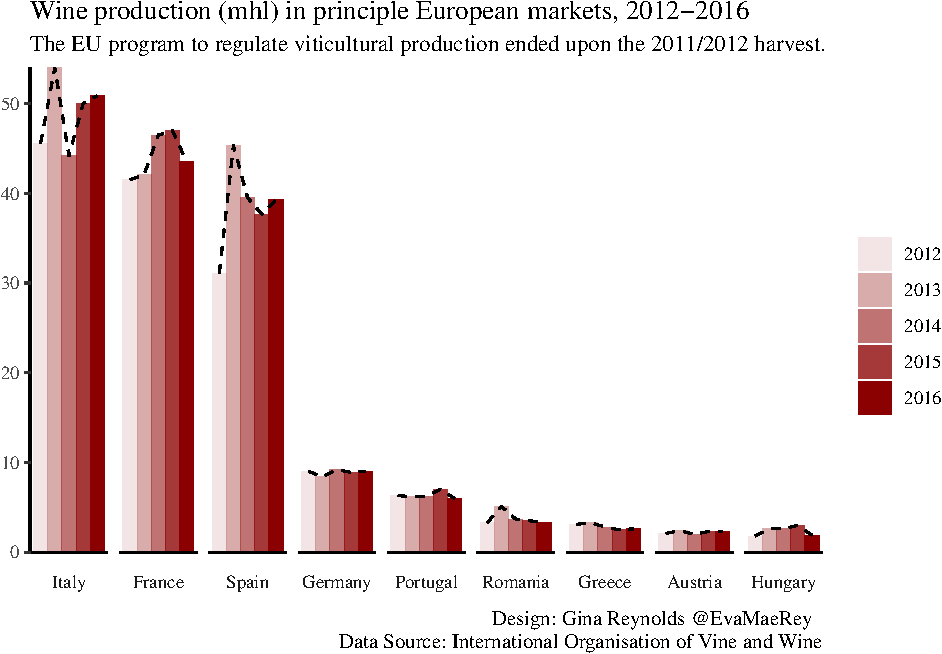
\includegraphics{makeovermonday_book_files/figure-latex/unnamed-chunk-50-1.pdf}

\chapter{Wine}\label{wine}

Wine production in Europe may have been volitile during the years
plotted because of production control policies implemented by the EU.
The big three, Italy, France and Spain, particularly saw a lot of
volitility early in this period.

\begin{Shaded}
\begin{Highlighting}[]
\NormalTok{df <-}\StringTok{ }\NormalTok{readxl}\OperatorTok{::}\KeywordTok{read_xlsx}\NormalTok{(}\StringTok{"raw_data/Wine_Production_by_country.xlsx"}\NormalTok{) }\OperatorTok
\StringTok{  }\KeywordTok{filter}\NormalTok{(Country }\OperatorTok{!=}\StringTok{ "World total"}\NormalTok{)}

\NormalTok{Europe <-}\StringTok{ }\KeywordTok{c}\NormalTok{(}
  \StringTok{"Italy"}\NormalTok{, }\StringTok{"France"}\NormalTok{, }\StringTok{"Spain"}\NormalTok{,}
  \StringTok{"Germany"}\NormalTok{, }\StringTok{"Portugal"}\NormalTok{, }\StringTok{"Romania"}\NormalTok{,}
  \StringTok{"Austria"}\NormalTok{, }\StringTok{"Greece"}\NormalTok{, }\StringTok{"Hungary"}
\NormalTok{)}
\end{Highlighting}
\end{Shaded}

\begin{Shaded}
\begin{Highlighting}[]
  \KeywordTok{ggplot}\NormalTok{(df }\OperatorTok\StringTok{ }\KeywordTok{filter}\NormalTok{(Country }\OperatorTok\StringTok{ }\NormalTok{Europe)) }\OperatorTok{+}
\StringTok{  }\KeywordTok{aes}\NormalTok{(}\DataTypeTok{x =}\NormalTok{ Year) }\OperatorTok{+}
\StringTok{  }\KeywordTok{aes}\NormalTok{(}\DataTypeTok{y =} \StringTok{`}\DataTypeTok{Wine production in mhl}\StringTok{`}\NormalTok{) }\OperatorTok{+}
\StringTok{  }\KeywordTok{facet_wrap}\NormalTok{(}\OperatorTok{~}\StringTok{ }\KeywordTok{fct_inorder}\NormalTok{(Country), }\DataTypeTok{strip.position =} \StringTok{"bottom"}\NormalTok{, }\DataTypeTok{nrow =} \DecValTok{1}\NormalTok{) }\OperatorTok{+}
\StringTok{  }\KeywordTok{geom_col}\NormalTok{(}\KeywordTok{aes}\NormalTok{(}\DataTypeTok{alpha =}\NormalTok{ Year), }\DataTypeTok{position =} \StringTok{"dodge"}\NormalTok{, }\DataTypeTok{fill =} \StringTok{"darkred"}\NormalTok{, }\DataTypeTok{width =} \DecValTok{1}\NormalTok{) }\OperatorTok{+}
\StringTok{  }\KeywordTok{geom_line}\NormalTok{(}\DataTypeTok{col =} \StringTok{"black"}\NormalTok{, }\DataTypeTok{lty =} \DecValTok{2}\NormalTok{) }\OperatorTok{+}
\StringTok{  }\KeywordTok{scale_y_continuous}\NormalTok{(}\DataTypeTok{expand =} \KeywordTok{c}\NormalTok{(}\DecValTok{0}\NormalTok{, }\DecValTok{0}\NormalTok{)) }\OperatorTok{+}
\StringTok{  }\KeywordTok{labs}\NormalTok{(}\DataTypeTok{fill =} \StringTok{""}\NormalTok{) }\OperatorTok{+}
\StringTok{  }\KeywordTok{labs}\NormalTok{(}\DataTypeTok{alpha =} \StringTok{""}\NormalTok{)}\OperatorTok{+}
\StringTok{  }\KeywordTok{labs}\NormalTok{(}\DataTypeTok{title =} \StringTok{"Wine production (mhl) in principle European markets, 2012-2016"}\NormalTok{) }\OperatorTok{+}
\StringTok{  }\KeywordTok{labs}\NormalTok{(}\DataTypeTok{subtitle =} \StringTok{"The EU program to regulate viticultural production ended upon the 2011/2012 harvest."}\NormalTok{) }\OperatorTok{+}\StringTok{ }
\StringTok{    }\KeywordTok{labs}\NormalTok{(}\DataTypeTok{caption =} \StringTok{"Design: Gina Reynolds @EvaMaeRey  }\CharTok{\textbackslash{}n}\StringTok{Data Source: International Organisation of Vine and Wine"}\NormalTok{) }\OperatorTok{+}\StringTok{ }\CommentTok{# \textbackslash{}nProduction volitility for top producers followed.}
\StringTok{  }\KeywordTok{theme_classic}\NormalTok{(}\DataTypeTok{base_family =} \StringTok{"Times"}\NormalTok{) }\OperatorTok{+}
\StringTok{  }\KeywordTok{theme}\NormalTok{(}
    \DataTypeTok{axis.title =} \KeywordTok{element_blank}\NormalTok{(),}
    \DataTypeTok{strip.placement =} \StringTok{"outside"}\NormalTok{,}
    \DataTypeTok{axis.text.x =} \KeywordTok{element_blank}\NormalTok{(),}
    \DataTypeTok{axis.ticks.x =} \KeywordTok{element_blank}\NormalTok{(),}
    \DataTypeTok{strip.background =} \KeywordTok{element_blank}\NormalTok{(),}
    \DataTypeTok{plot.caption =} \KeywordTok{element_text}\NormalTok{(}\DataTypeTok{size =} \DecValTok{10}\NormalTok{)}
\NormalTok{  )}
\end{Highlighting}
\end{Shaded}

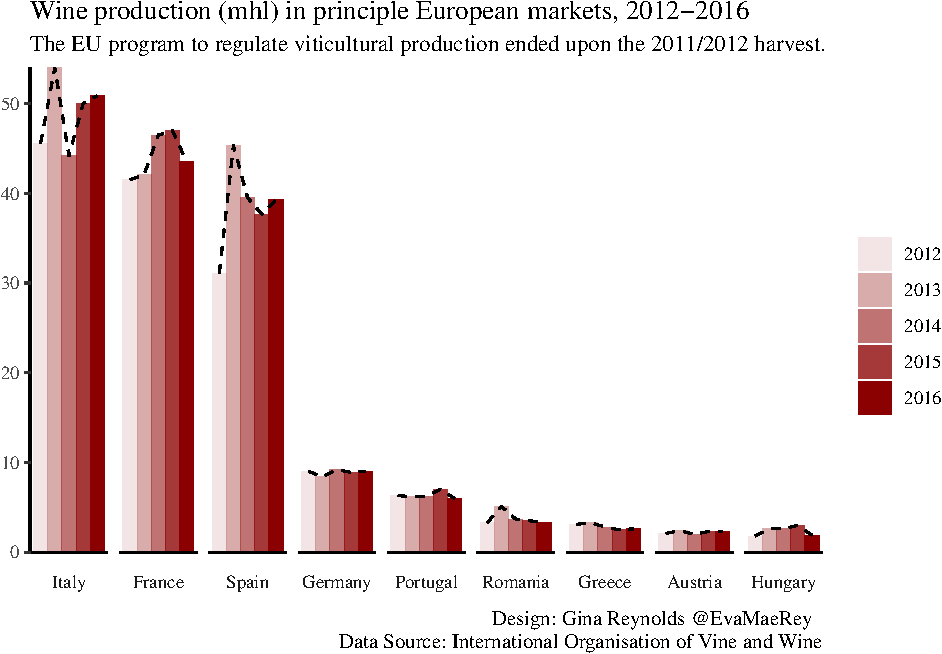
\includegraphics{makeovermonday_book_files/figure-latex/unnamed-chunk-52-1.pdf}

\chapter{Arctic Ice}\label{arctic-ice}

This visualization shows the trend in Arctic Ice Sea Extent, data from
the National Snow and Ice Data Center. If I recall correctly, the
definition for coverage is the case where at least 15 percent of the sea
is ice.

The visualization shows melting and freezing cycles, in accordance with
the seasons --- and the disconcerting trend of a general decrease in ice
extent over the years.

One problem that arises is due to inconsistant number of days in each
year. There is a measurement for every day, but leap years contain a
extra day. Which means that plotting years over years leads to imperfect
alignment. My solution was just to pretend that all the data come from a
single year, 2000, and plot each of the years on that scale. The
earliest year cycle and last year cycle are highlighted in white.

A random sample from the data set:

\begin{tabular}{l|r|r|l|l|r|r|r}
\hline
Date & Extent (million sq km) & year & month\_day & month\_day\_plus & proportion\_ocean\_covered\_in\_ice & mean\_for\_day & diff\_from\_mean\_day\\
\hline
1998-05-10 & 13.991 & 1998 & 05-10 & 2000-05-10 & 0.0388639 & 13.432771 & 0.5582286\\
\hline
1989-02-24 & 15.638 & 1989 & 02-24 & 2000-02-24 & 0.0434389 & 15.262353 & 0.3756471\\
\hline
1988-01-25 & 15.020 & 1988 & 01-25 & 2000-01-25 & 0.0417222 & 14.568265 & 0.4517353\\
\hline
2008-09-04 & 4.686 & 2008 & 09-04 & 2000-09-04 & 0.0130167 & 5.977629 & -1.2916286\\
\hline
1984-07-06 & 10.807 & 1984 & 07-06 & 2000-07-06 & 0.0300194 & 9.969500 & 0.8375000\\
\hline
\end{tabular}

\begin{tabular}{r|r|r|l}
\hline
year & average\_coverage & num\_days & average\_day\\
\hline
1982 & 12.43945 & 182 & 1982-07-02 00:00:00\\
\hline
2016 & 10.15069 & 366 & 2016-07-01 12:00:00\\
\hline
\end{tabular}

\begin{Shaded}
\begin{Highlighting}[]
\CommentTok{# breaks for x axis.}
\NormalTok{br <-}\StringTok{ }\KeywordTok{as.numeric}\NormalTok{(lubridate}\OperatorTok{::}\KeywordTok{ymd}\NormalTok{(}\KeywordTok{c}\NormalTok{(}
  \StringTok{"2000-01-01"}\NormalTok{, }\StringTok{"2000-04-01"}\NormalTok{,}
  \StringTok{"2000-07-01"}\NormalTok{, }\StringTok{"2000-10-01"}\NormalTok{, }\StringTok{"2001-01-01"}
\NormalTok{)))}

\KeywordTok{ggplot}\NormalTok{(df) }\OperatorTok{+}
\StringTok{  }\KeywordTok{aes}\NormalTok{(}\DataTypeTok{x =} \KeywordTok{as.numeric}\NormalTok{(month_day_plus)) }\OperatorTok{+}
\StringTok{  }\KeywordTok{aes}\NormalTok{(}\DataTypeTok{y =} \StringTok{`}\DataTypeTok{Extent (million sq km)}\StringTok{`}\NormalTok{) }\OperatorTok{+}
\StringTok{  }\KeywordTok{aes}\NormalTok{(}\DataTypeTok{group =}\NormalTok{ year) }\OperatorTok{+}
\StringTok{  }\KeywordTok{geom_line}\NormalTok{() }\OperatorTok{+}
\StringTok{  }\KeywordTok{aes}\NormalTok{(}\DataTypeTok{col =}\NormalTok{ year) }\OperatorTok{+}
\StringTok{  }\KeywordTok{scale_x_continuous}\NormalTok{(}
    \DataTypeTok{breaks =}\NormalTok{ br,}
    \DataTypeTok{labels =} \KeywordTok{c}\NormalTok{(}\StringTok{"Jan-01"}\NormalTok{, }\StringTok{"Apr-01"}\NormalTok{, }\StringTok{"Jul-01"}\NormalTok{, }\StringTok{"Oct-01"}\NormalTok{, }\StringTok{"Jan-01"}\NormalTok{), }
    \DataTypeTok{expand =} \KeywordTok{c}\NormalTok{(}\DecValTok{0}\NormalTok{, }\DecValTok{0}\NormalTok{)}
\NormalTok{  ) }\OperatorTok{+}
\StringTok{  }\KeywordTok{scale_y_continuous}\NormalTok{(}\DataTypeTok{expand =} \KeywordTok{c}\NormalTok{(}\DecValTok{0}\NormalTok{, }\DecValTok{0}\NormalTok{), }\DataTypeTok{limits =} \KeywordTok{c}\NormalTok{(}\DecValTok{0}\NormalTok{, }\DecValTok{20}\NormalTok{)) }\OperatorTok{+}
\StringTok{  }\KeywordTok{scale_color_continuous}\NormalTok{(}
    \DataTypeTok{guide =} \KeywordTok{guide_colourbar}\NormalTok{(}\DataTypeTok{reverse =} \OtherTok{TRUE}\NormalTok{),}
    \DataTypeTok{breaks =} \KeywordTok{seq}\NormalTok{(}\DecValTok{2010}\NormalTok{, }\DecValTok{1980}\NormalTok{, }\OperatorTok{-}\DecValTok{10}\NormalTok{)}
\NormalTok{  ) }\OperatorTok{+}
\StringTok{  }\KeywordTok{geom_line}\NormalTok{(}\KeywordTok{aes}\NormalTok{(}\DataTypeTok{lty =} \KeywordTok{factor}\NormalTok{(year)),}
    \DataTypeTok{data =}\NormalTok{ df }\OperatorTok\StringTok{ }\KeywordTok{filter}\NormalTok{(year }\OperatorTok{==}\StringTok{ }\DecValTok{2016} \OperatorTok{|}\StringTok{ }\NormalTok{year }\OperatorTok{==}\StringTok{ }\DecValTok{1982}\NormalTok{),}
    \DataTypeTok{col =} \StringTok{"white"}
\NormalTok{  ) }\OperatorTok{+}
\StringTok{  }\KeywordTok{scale_linetype_manual}\NormalTok{(}
    \DataTypeTok{name =} \StringTok{""}\NormalTok{,}
    \DataTypeTok{values =} \KeywordTok{c}\NormalTok{(}\StringTok{"dashed"}\NormalTok{, }\StringTok{"solid"}\NormalTok{)}
\NormalTok{  ) }\OperatorTok{+}
\StringTok{  }\KeywordTok{annotate}\NormalTok{(}
    \DataTypeTok{geom =} \StringTok{"text"}\NormalTok{, }\DataTypeTok{x =} \DecValTok{11210}\NormalTok{, }\DataTypeTok{y =} \DecValTok{15}\NormalTok{,}
    \DataTypeTok{label =} \KeywordTok{str_wrap}\NormalTok{(}\StringTok{"For this period, 1982 had the highest calendar-year average extent of Arctic sea ice while 2016 had the lowest"}\NormalTok{, }\DecValTok{30}\NormalTok{),}
    \DataTypeTok{col =} \StringTok{"white"}\NormalTok{,}
    \DataTypeTok{size =} \DecValTok{7}
\NormalTok{  ) }\OperatorTok{+}
\StringTok{  }\KeywordTok{labs}\NormalTok{(}\DataTypeTok{x =} \StringTok{""}\NormalTok{) }\OperatorTok{+}
\StringTok{  }\KeywordTok{labs}\NormalTok{(}\DataTypeTok{y =} \StringTok{"extent (million sq km)"}\NormalTok{) }\OperatorTok{+}
\StringTok{  }\KeywordTok{labs}\NormalTok{(}\DataTypeTok{col =} \StringTok{""}\NormalTok{) }\OperatorTok{+}
\StringTok{  }\KeywordTok{labs}\NormalTok{(}\DataTypeTok{lty =} \StringTok{""}\NormalTok{) }\OperatorTok{+}
\StringTok{  }\KeywordTok{labs}\NormalTok{(}\DataTypeTok{title =} \StringTok{"Freezing cycles: Arctic sea ice extent, 1979-2017"}\NormalTok{) }\OperatorTok{+}
\StringTok{  }\KeywordTok{labs}\NormalTok{(}\DataTypeTok{subtitle =} \StringTok{"Data Source: National Snow & Ice Data Center | Vis: Gina Reynolds for #MakeoverMonday"}\NormalTok{) }\OperatorTok{+}
\StringTok{  }\KeywordTok{theme_dark}\NormalTok{(}\DataTypeTok{base_size =} \DecValTok{14}\NormalTok{) }\OperatorTok{+}
\StringTok{  }\KeywordTok{theme}\NormalTok{(}
    \DataTypeTok{legend.background =} \KeywordTok{element_blank}\NormalTok{(),}
    \DataTypeTok{legend.position =} \KeywordTok{c}\NormalTok{(}\FloatTok{0.1}\NormalTok{, .}\DecValTok{35}\NormalTok{),}
    \DataTypeTok{legend.text =} \KeywordTok{element_text}\NormalTok{(}\DataTypeTok{colour =} \StringTok{"white"}\NormalTok{, }\DataTypeTok{size =} \DecValTok{15}\NormalTok{),}
    \DataTypeTok{plot.background =} \KeywordTok{element_rect}\NormalTok{(}\DataTypeTok{fill =} \StringTok{"grey30"}\NormalTok{),}
    \DataTypeTok{plot.title =} \KeywordTok{element_text}\NormalTok{(}\DataTypeTok{colour =} \StringTok{"lightgrey"}\NormalTok{),}
    \DataTypeTok{plot.subtitle =} \KeywordTok{element_text}\NormalTok{(}\DataTypeTok{colour =} \StringTok{"lightgrey"}\NormalTok{),}
    \DataTypeTok{axis.title =} \KeywordTok{element_text}\NormalTok{(}\DataTypeTok{colour =} \StringTok{"lightgrey"}\NormalTok{),}
    \DataTypeTok{axis.line =} \KeywordTok{element_line}\NormalTok{(}\DataTypeTok{colour =} \StringTok{"lightgrey"}\NormalTok{),}
    \DataTypeTok{axis.text =} \KeywordTok{element_text}\NormalTok{(}\DataTypeTok{colour =} \StringTok{"lightgrey"}\NormalTok{),}
    \DataTypeTok{axis.ticks =} \KeywordTok{element_line}\NormalTok{(}\DataTypeTok{colour =} \StringTok{"lightgrey"}\NormalTok{)}
\NormalTok{  )}
\end{Highlighting}
\end{Shaded}

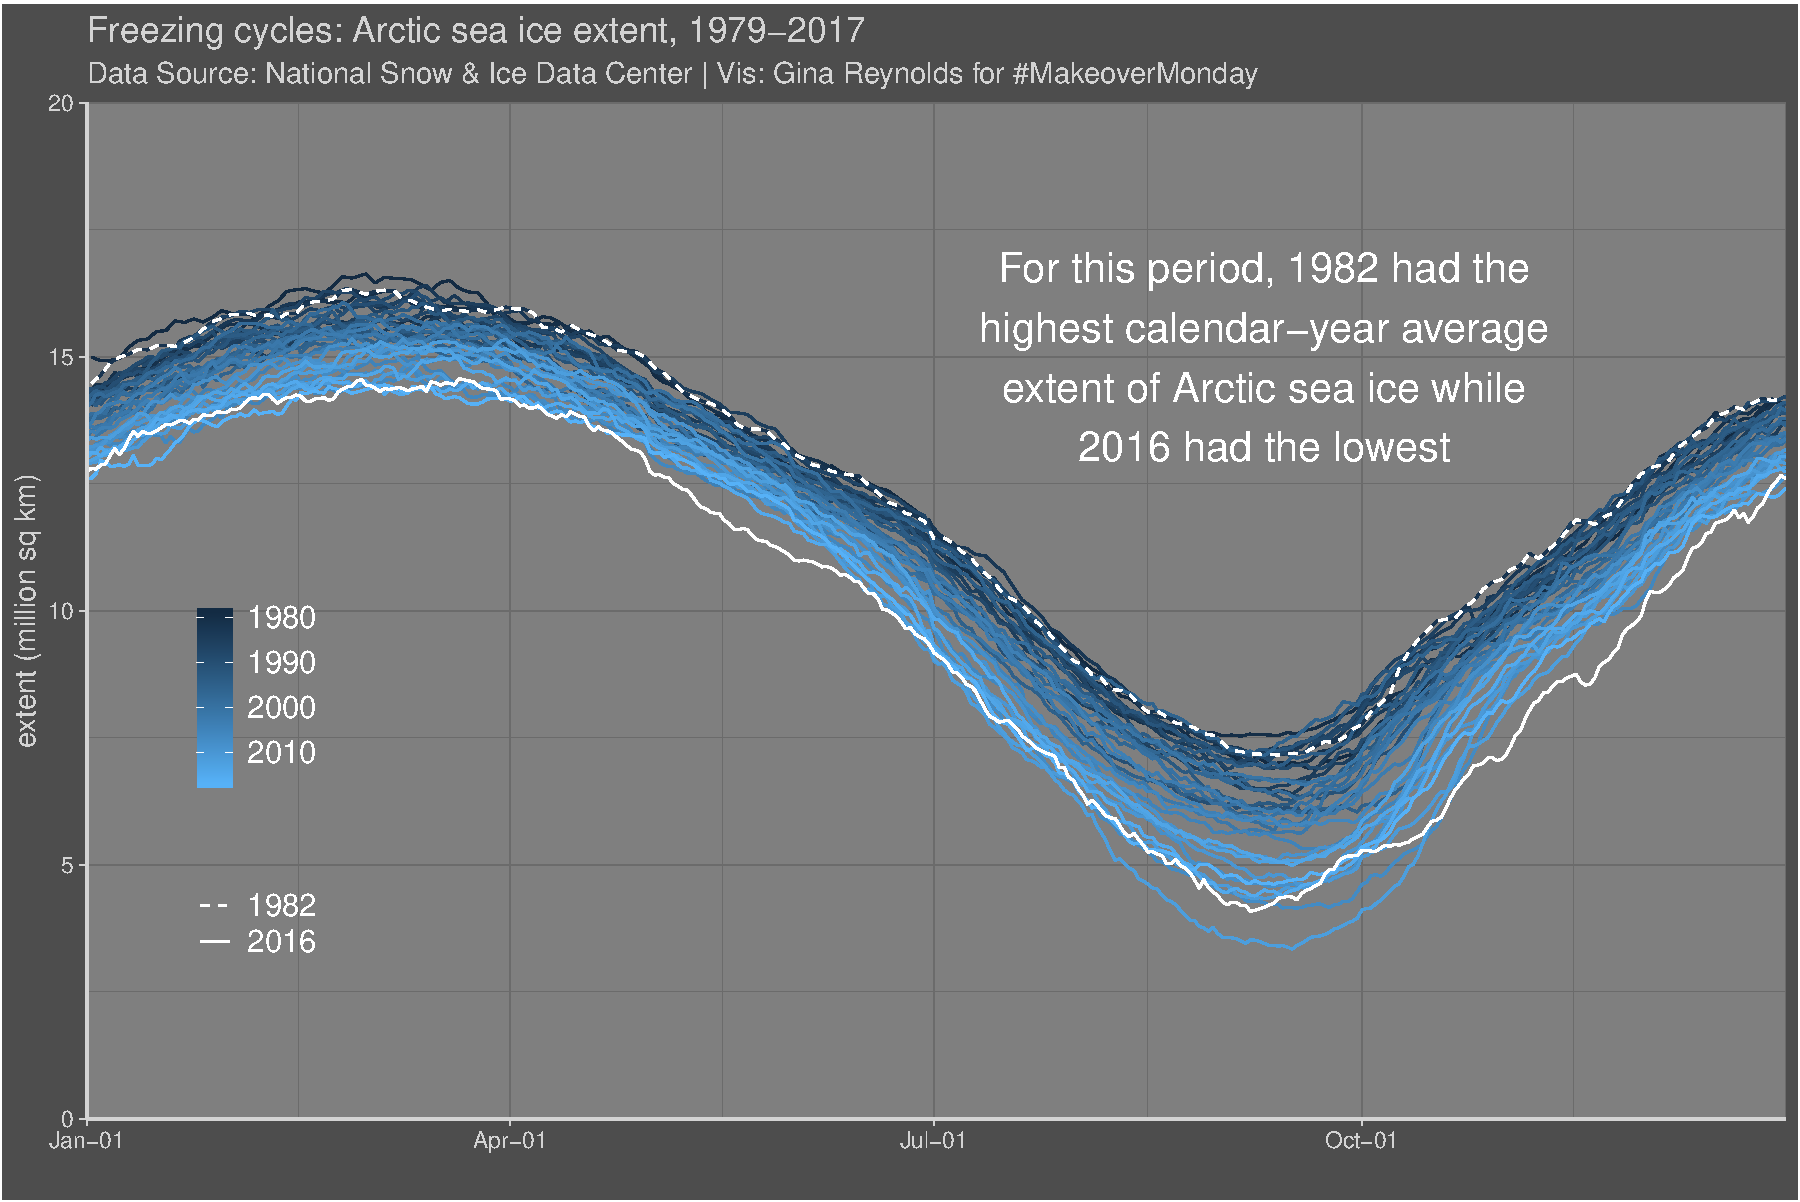
\includegraphics{makeovermonday_book_files/figure-latex/unnamed-chunk-56-1.pdf}

\bibliography{book.bib,packages.bib}


\end{document}
